\documentclass[11pt,twoside]{article}
\usepackage{geometry}
\usepackage{enumerate}
\usepackage{latexsym,booktabs}
\usepackage{amsmath,amssymb}
\usepackage{graphicx}
\usepackage{hyperref}
\usepackage[singlespacing]{setspace}
\usepackage{calc}
\usepackage{blindtext}
\usepackage{subfig}
\usepackage{graphicx}
\usepackage{tikz}
\usetikzlibrary{positioning}

\geometry{a4paper,left=2cm,right=2.0cm, top=2cm, bottom=2.0cm}

\newtheorem{Definition}{Definition}
\newtheorem{Theorem}{Theorem}
\newtheorem{Lemma}{Lemma}
\newtheorem{Corollary}{Corollary}
\newtheorem{Proposition}{Proposition}
\newtheorem{Algorithm}{Algorithm}
\numberwithin{Theorem}{section}
\numberwithin{Definition}{section}
\numberwithin{Lemma}{section}
\numberwithin{Algorithm}{section}
\numberwithin{equation}{section}

\newcommand{\dottedline}[1]{\makebox[#1]{.\dotfill}}

\begin{document}

\pagestyle{empty}

% =============================================================================
% Title page
% =============================================================================
\begin{titlepage}
\vspace*{.5em}
\center
\textbf{\Large{The School of Mathematics}} \\
\vspace*{1em}
\begin{figure}[!h]
\centering

\includegraphics[width=180pt]{CentredLogoCMYK.jpg}
\end{figure}
\vspace{2em}
\textbf{\Huge{Anomaly Detection with Bayesian Neural Networks}}\\[2em]
\textbf{\LARGE{by}}\\
\vspace{2em}
\textbf{\LARGE{Theodoros Ladas}}\\
\vspace{6.5em}
\Large{Dissertation Presented for the Degree of\\
MSc in Statistics with Data Science}\\
\vspace{6.5em}
\Large{July 2021}\\
\vspace{3em}
\Large{Supervised by\\Dr Bruce Worton and Dr Daniel Paulin}
\vfill
\end{titlepage}

\cleardoublepage

% =============================================================================
% Executive summary, acknowledgments, and own work declaration
% =============================================================================
\begin{center}
\Large{Executive Summary}
\end{center}

Here comes your executive summary ...

\clearpage

\begin{center}
\Large{Acknowledgments}
\end{center}

Here come your acknowledgments ...

\clearpage

\begin{center}
\Large{University of Edinburgh – Own Work Declaration}
\end{center}


This sheet must be filled in, signed and dated - your work will not be marked unless this is done.
\vspace{1cm}

Name: \dottedline{8cm}

Matriculation Number: \dottedline{6cm}

Title of work: \dottedline{8cm}

\vspace{1cm}

I confirm that all this work is my own except where indicated, and that I have:
\begin{itemize}
\item	Clearly referenced/listed all sources as appropriate	 				
\item	Referenced and put in inverted commas all quoted text (from books, web, etc)	
\item	Given the sources of all pictures, data etc. that are not my own				
\item	Not made any use of the report(s) or essay(s) of any other student(s) either past 	
or present	
\item	Not sought or used the help of any external professional academic agencies for the work
\item	Acknowledged in appropriate places any help that I have received from others	(e.g. fellow students, technicians, statisticians, external sources)
\item	Complied with any other plagiarism criteria specified in the Course handbook
\end{itemize}

I understand that any false claim for this work will be penalised in accordance with
the University regulations	(\url{https://teaching.maths.ed.ac.uk/main/msc-students/msc-programmes/statistics/data-science/assessment/academic-misconduct}).								

\vspace{1cm}

Signature \dottedline{8cm}

\vspace{5mm}

Date \dottedline{8cm}


\clearpage



% =============================================================================
% Table of contents, tables, and pictures (if applicable)
% =============================================================================
\pagestyle{plain}
\setcounter{page}{1}
\pagenumbering{Roman}

\tableofcontents
\clearpage
\listoftables
\listoffigures
\cleardoublepage

\pagenumbering{arabic}
\setcounter{page}{1}

\nocite{*}
\bibliographystyle{abbrv}
\clearpage

% ------------------------------------------------------------------------------------------------------
\section{Introduction}

\subsection{Motivation}
\label{sec:motivation}
Anomaly detection is a very useful technique, leveraged (among others) by the banking sector in order to automaticaly block fraudulent transactions. This dissertation project is a detailed explanation of how an anomaly detection system could be implemented using Bayesian neural networks. This application, uses machine learning to train a model on a set of data, in order to predict an outcome of interest. Afterwards, the predictions are drawn many times (bootstraped), in order to create an estimation of confidence about the prediction. The goal of the project is to automatically flag transactions that could be fraudulent, thus allowing a human to spend time in deep investigation of those transactions, rather than manually going through each transaction one by one. 

This report is divided into the \textit{Introduction}, \textit{Exploratory Data Analysis}, \textit{Methods}, and \textit{Results} sections and a brief summary of each one is presented here. The rest of the \textit{Introduction} section will explain the specific dataset used for the presentation of the problem, as well as all the software requirements to be able to reproduce the results. Next, the \textit{Exploratory Data Analysis} section, presents a various aspects of the data, such as the distributions of the features, their corelations as well as a quick way to visually discover potential anomalies. On the \textit{Methods} section, the specific architecture of all the neural netwokrs models are presented, as well as the way the best model was selected (model validation). Finaly, three related but different metrics are presented in the \textit{Results} section of what constitutes as an anomaly, yet the specific threshhold for those metrics, is arbitrarily set. In a real life application this is a business decision, that should be set by the stakeholders according to their criteria. 

\subsection{Data Sources}
\label{sec:back}
The dataset used in this project, was given by the University of Edinburgh in the context of the dissertation project and it is the wine dataset. It is an especially clean and very well known real-life dataset for prototype creation. The basic assumption is that if the algorithm manages to capture anomalies on this dataset, it is in principal possible to productionise a variant of the architecture for an application of interest. More specifically it is a 4898 (rows) $\times$ 12 (columns) matrix, with no missing values and no duplicated rows. Each row represents one wine and the columns are the various features of each wine, such as its degrees of \textit{alcohol}, the \textit{acidity} of the wine, the \textit{pH} level wich measures how acidic or basic the solution etc. The problem this dissertation is going to try to solve, is a classification problem, of the \textit{type} of the wine, according to all other features. The variable \textit{type} is either \textit{1, 2, or 3} and the classes are almost perfectly balance thus making easier the preprocessing stage of the problem, and focusing more on the architecture and the interpretation of the algorithm as well as its results. Thus, the only preprocessing steps needed are the centering and scaling of the data matrix, to ensure that variables can potentially have the same impact regardless of the scale they are measured in and one-hot encoding the \textit{quality} feature, since its also not a numeric variable, but a factor one. Lastly, The dataset is split into train ($80\%$), validation ($25\%$) and test ($25\%$) sets to ensure that no algorithm overfits the given dataset. 

\subsection{Software}
\label{sec:software}
A combination of the programming languages \textsf{R} and \textsf{Python} are used to produce this report. The use of both languages is in no way binding. \textsf{R} is used for the exploration of the dataset, as well as for the dimensionality reduction plots, while \textsf{Python} is used in combination with \textsf{tensorflow},\textsf{tensorflow-probability}, and \textsf{keras} to build, validate, and test the neural networks. These packages can also be used from the \textsf{R} ecosystem, yet the setup process is more complicated and thus avoided. The reason \textsf{R} is selected for the EDA, is due to the \textsf{ggplot2} package, wich is a very powerfull and easy package for creating complicated plots.
\clearpage


%------------------------------------------------------------------------------------------------------
\section{Exploratory Data Analysis}
In this section a basic overview of the dataset and its properties is going to be presented. Firstly, various statistics regarding the dataset are presented in the form of graphs, in univariate, bivariate and multivariate analysis. Afterwards, the dataset it reduced in dimensions with two techniques (a linear and a non-linear) in order to be able to plot it with a two-dimensional graph. This is also a quick way to identify potential anomalies as well visually. The reason of the extended EDA, is to understand what preprocessing steps could be needed in order for the future models to work correctly. Also, the knowledge gained from this exploration of the dataset will help in the explanation of the model in the \textit{Model Validation} section. 

\subsection{Univatiate Analysis}
\label{sec:univariate}
The dataset, consist of twelve feature variables, out of which only one (\textit{quality}) is categorical, while all the others are numeric. The target varaiable (\textit{type}) is also a target variable with three levels \textsf{type=1, type=2, type=3}. There are no missing values.

\vspace*{1em}
\begin{figure}[!h]
\centering
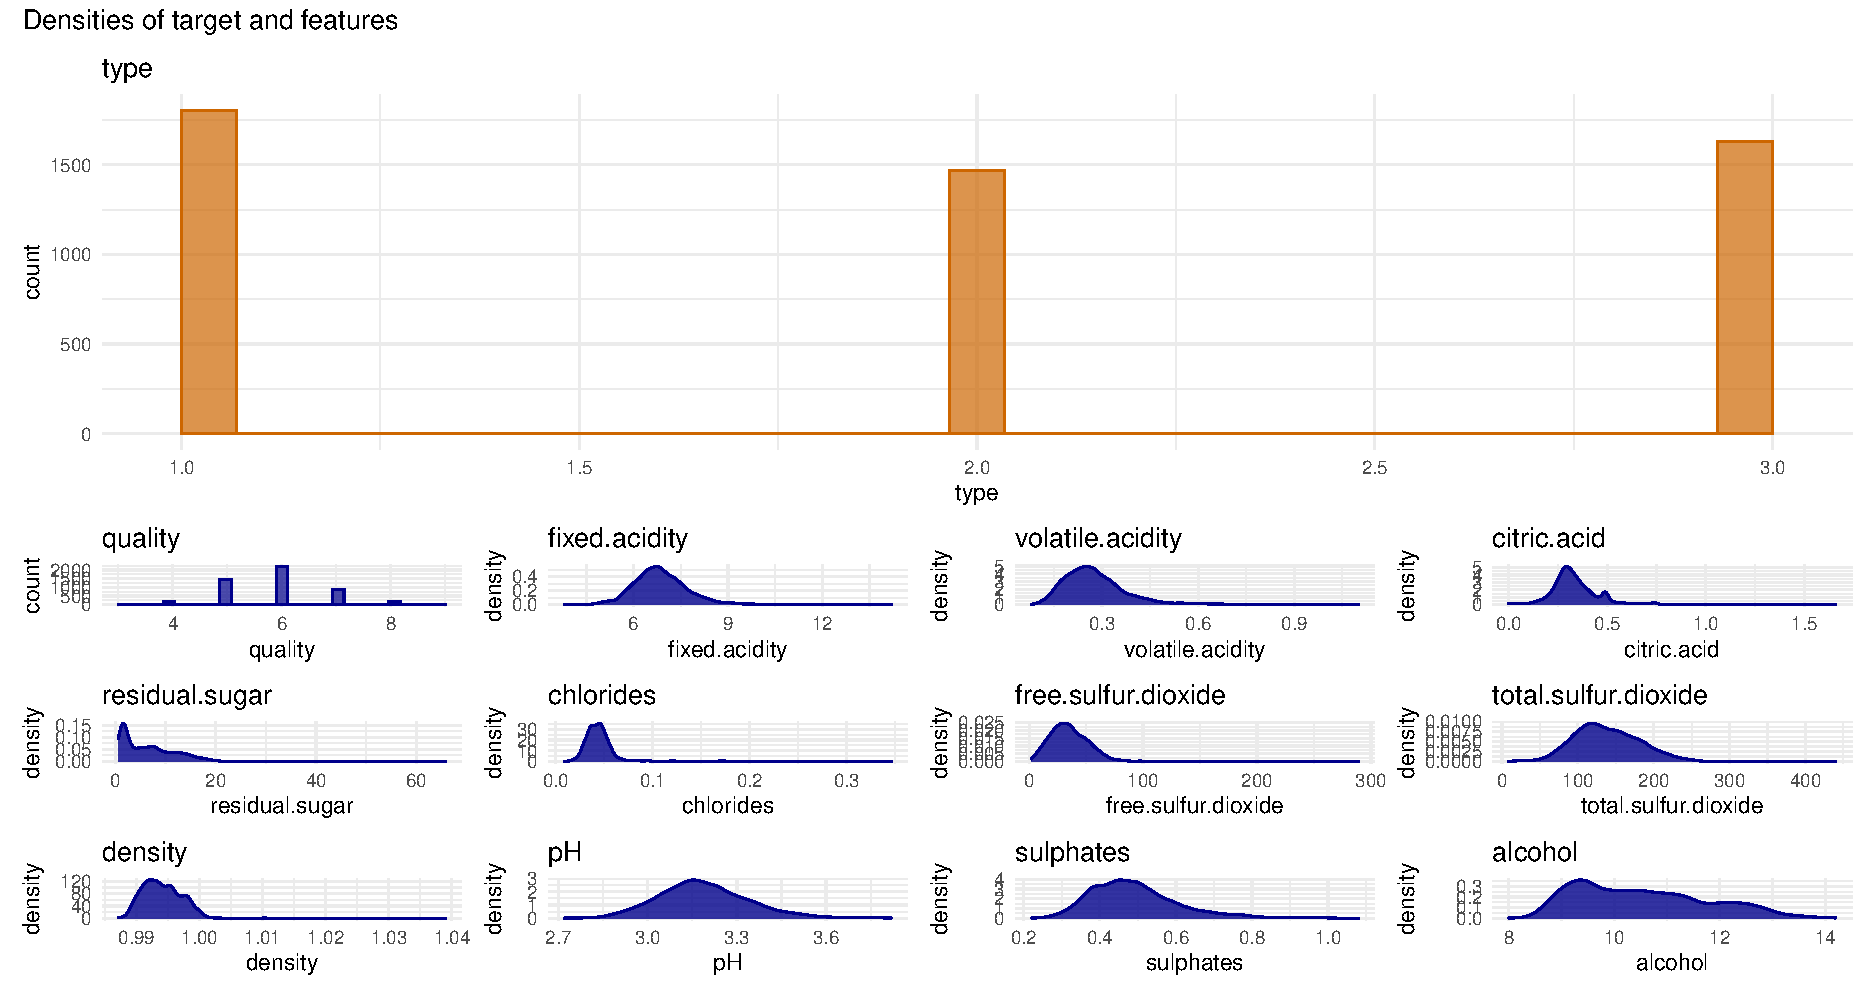
\includegraphics[width=\textwidth]{./output/1.h.univariate-analysis.pdf}
\caption{centered image}
\label{fig:uni}
\end{figure}
\vspace{2em}

In \autoref{fig:uni}, the target variable type is represented by the orange barplot. The number of rows in each class is balanced therefore no preprocessing to upsample (downsample) the underepresented (overrepresented) classes is needed. On the variable \textit{quality}, the majority of cases are \\
 $(quality\geq5) \lor (quality\leq7)$, which would make the very poor and very good wines difficult to predict. Finally, evidently the features, are measured in vastly different scales. For example \textit{pH} is ranging from 2.7 to 3.6, while \textit{free.residual.dioxide} is ranging from 0 to 300. This means that centering and scaling the data matrix is crusial for any algorithm to work properly.

\subsection{Bivariate Analysis}
\label{sec:bivariate}

Extending the univariate analysis of the previous subsection, the bivariate analysis reveals how the features correlate to each other. \autoref{fig:corr} (a) and \autoref{fig:corr} (b) are both producing the same information but presented differently. On \autoref{fig:corr} (a) the exact values of the linear relationships are shown, while on \autoref{fig:corr} (b) clear clusters of high and low linear correlation are formed. Out of these clusters that are present in \autoref{fig:corr} (b) some are expected but others are not.

For measuring the correaltion, the \textit{Pearson's correlation coefficient} is used, which measures the covariance of two random variables, $X$ and $Y$, and normalizes it with the product of their standard deviations, or:

\begin{equation}
\rho(x,y) = \frac{\text{cov}(x,y)}{\text{std}(x)\text{std}(y)}
\end{equation}

\begin{figure}[h]
    \centering
    \subfloat[Correlation matrix]
    {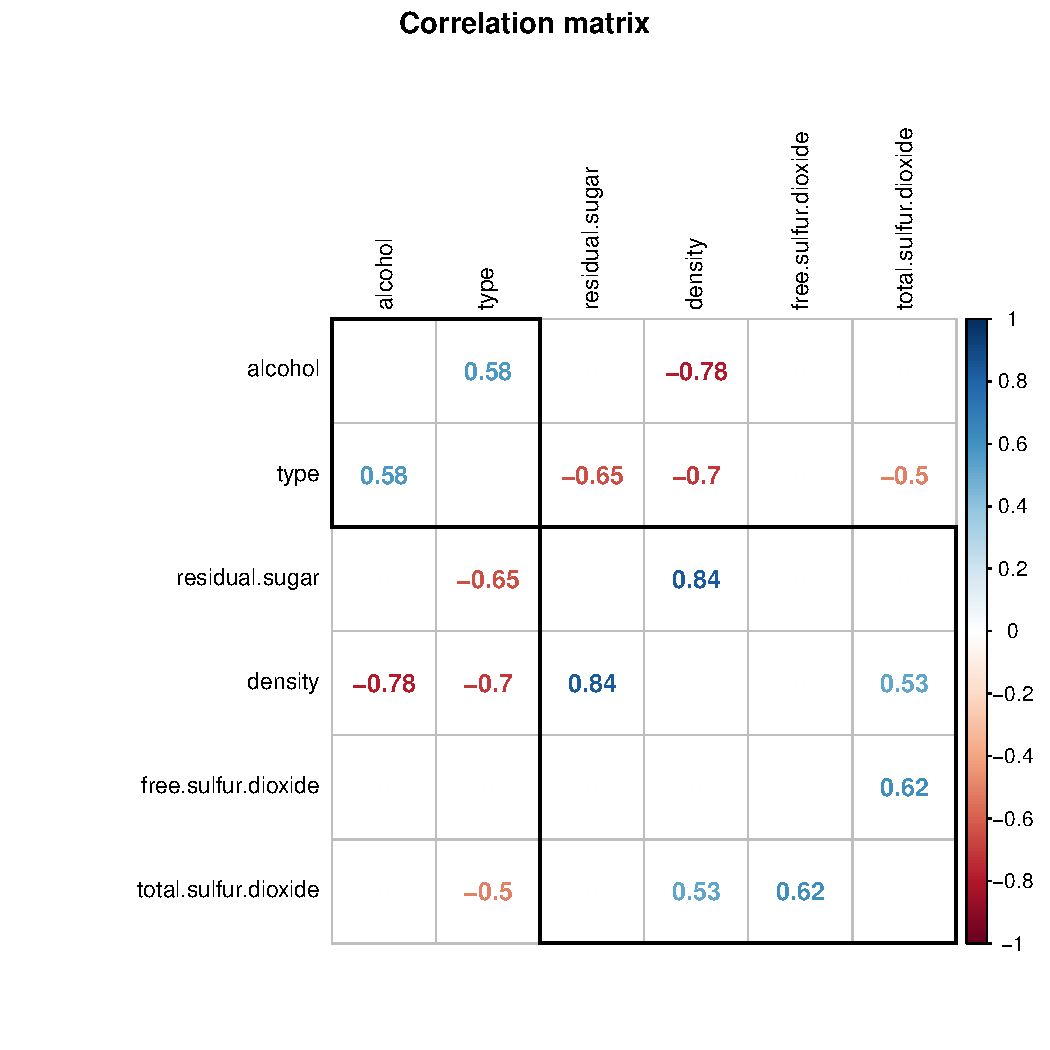
\includegraphics[width=.4\textwidth,height=.25\textheight]{./output/1.e.corrplot-1.pdf}}
    \subfloat[Correlation network]
    {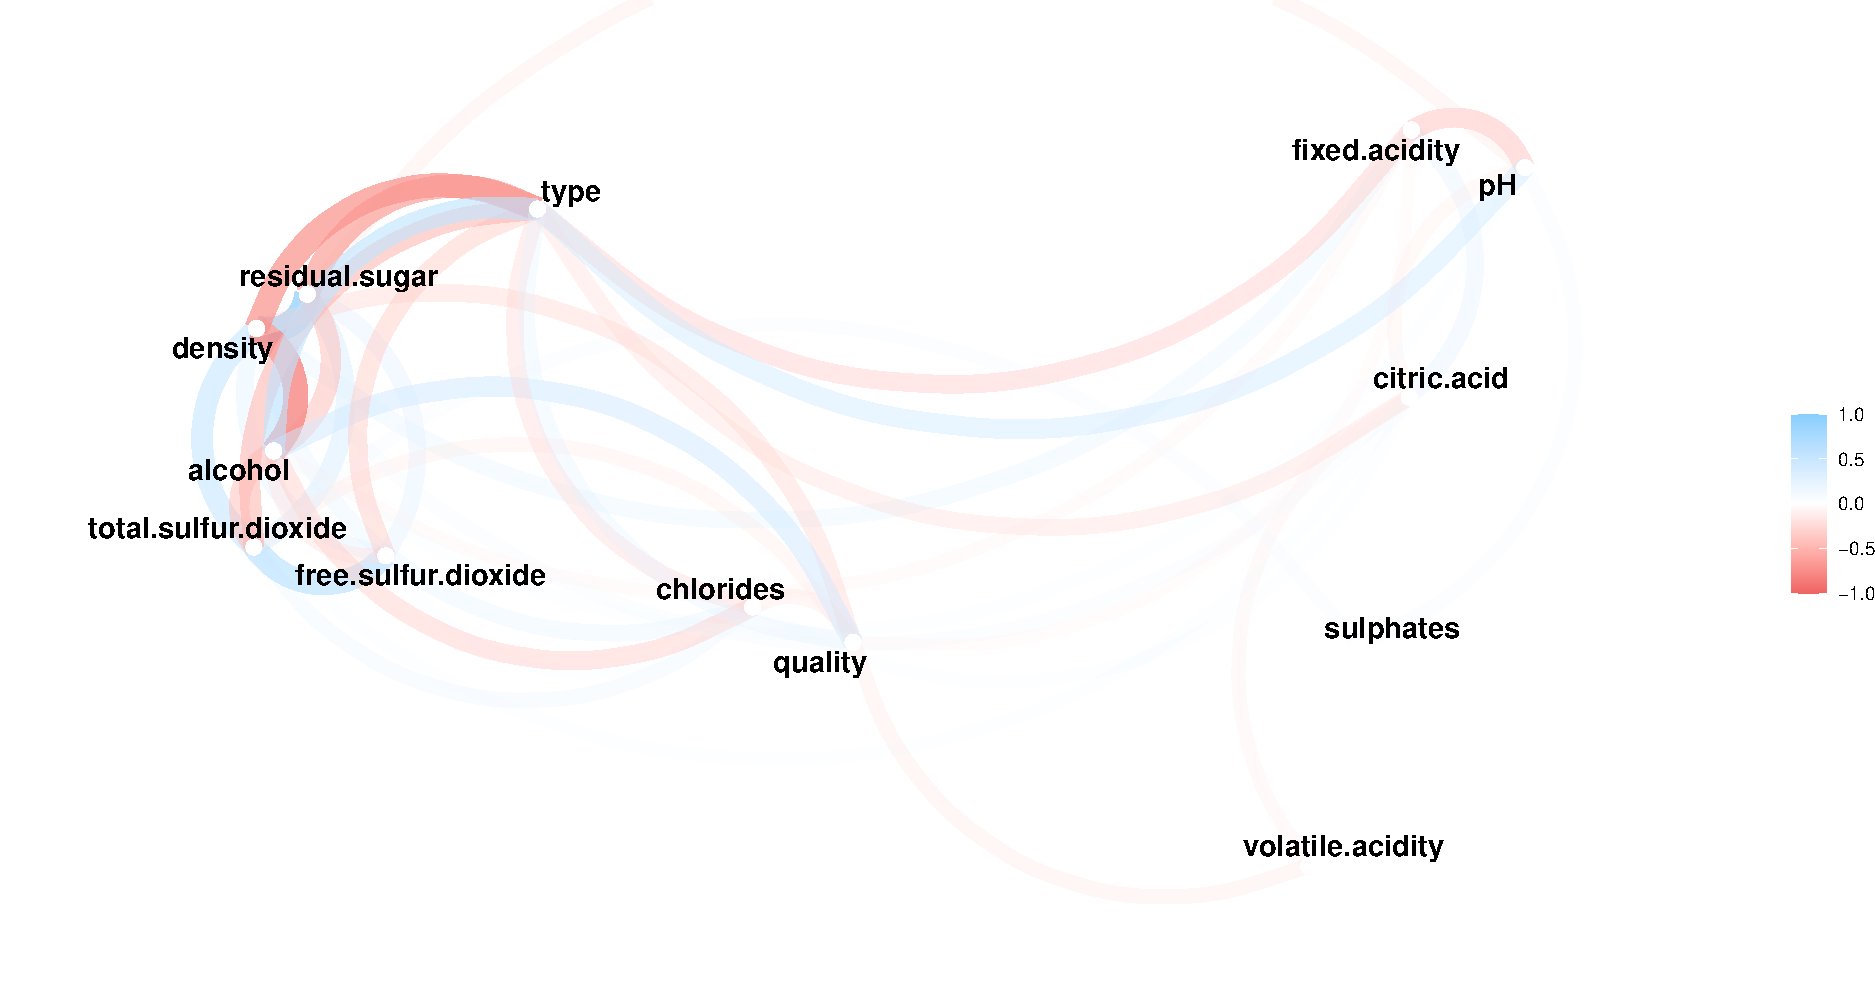
\includegraphics[width=.6\textwidth]{./output/1.f.corplot-2.pdf}}
    \caption{}
    \label{fig:corr}
\end{figure}

For example, \autoref{fig:corr} (a) shows a strong positive relationship between \textit{free.sulfur.dioxide} and \textit{total.sulfur.dioxide}, which is expected, as \textit{total.sulfur.dioxide} is the \textit{free.sulfur.dioxide} plus other sulfur dioxides from other ingredients. Intrestingly, the same is not true regarding \textit{volatile.acidity}, \textit{fixed.acidity} and \textit{citric.acid}. The feature with the most strong correlations however, is \textit{density}, as it strongly correlates, both positively or negatively with \textit{alcohol}, \textit{type}, \textit{residual.sugar} and \textit{total.sulfur.dioxide}. 

In general we identify two clusters. One with strong correlations containing \textit{type}, \textit{residual.sugar}, \textit{density}, \textit{alcohol}, \textit{total.sulfure.dioxide} and \textit{free.sulfure.dioxide}, and a second one with low correlations containing \textit{fixed.acidity}, \textit{pH}, \textit{citric.acid}, \textit{sulphates} and \textit{volatile.acidity}. The model is going to leverage this relationships in order to predict the outcome. 

\subsection{Dimensionality Reduction}
\label{sec:reduction}
In the exploration of the dataset, two different techniques were used in order to reduce the dimensions and visualize it with plots. The first method is the Principal Component Analysis (PCA), which a singular value decomposition (SVD) of the centered, data matrix. The SVD of an $ m \times n $ matrix $A$ is the factorization of the matrix into $USV^\top$. Secondly, a more advanced nonlinear dimensionality reduction method, called t-distributed Stochastic Neighbor Embedding (t-SNE) was tryied, to cross evaluate the results of PCA. This methods works by finding a way to project the high dimensional data into a lower dimension, while preserving the culstering of the higher dimension.

\subsubsection{PCA}
\label{sec:pca}

Using the singular value decomposition to factorize the data matrix $X$, we produce, three matrixes, $U$, $S$ and $V$, each carrying information about the dataset in some aspect. First of all, we can create the following graph of the percentage of variance explained by each principal component. 
%----------
\vspace*{1em}
\begin{figure}[!h]
\centering
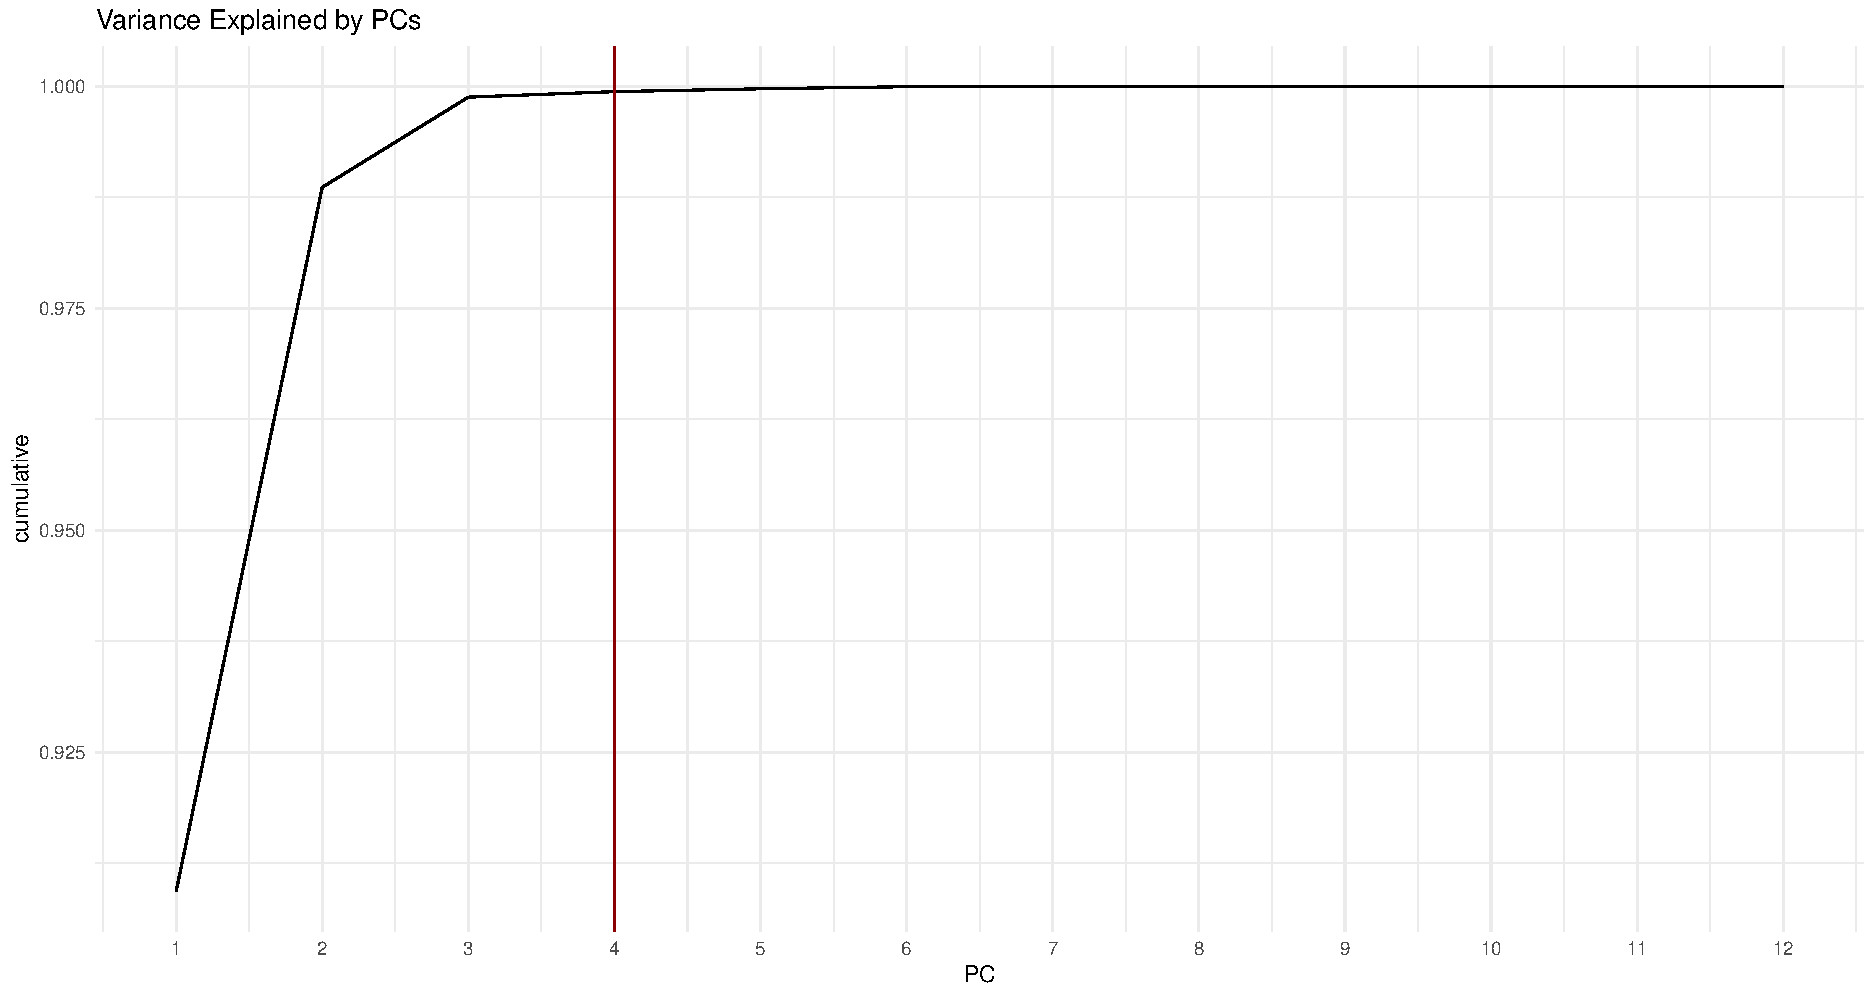
\includegraphics[width=\textwidth]{./output/1.a.pca-var-expl.pdf}
\caption{}
\label{fig:var_expl}
\end{figure}
\vspace{2em}
%----------

In \autoref{fig:var_expl}, we can see the cummalative variance explained by each additional principal component. This is a very important graph as we can reduce the dimension of the data matrix by selecting a threshold (for example, 99\% of the variance). In this example, it is clear that with only the first four principal components, that threshold is surpassed.

The principal components are a linear compination of all the columns of the dataset, and each one is perpandicular to the previous one. We can continue the exploration by visualizing the weights (loadings) of these four principal components and try to understand wheather these components make sense according to our knowledge on the topic. 

%----------
\vspace*{1em}
\begin{figure}[!h]
\centering
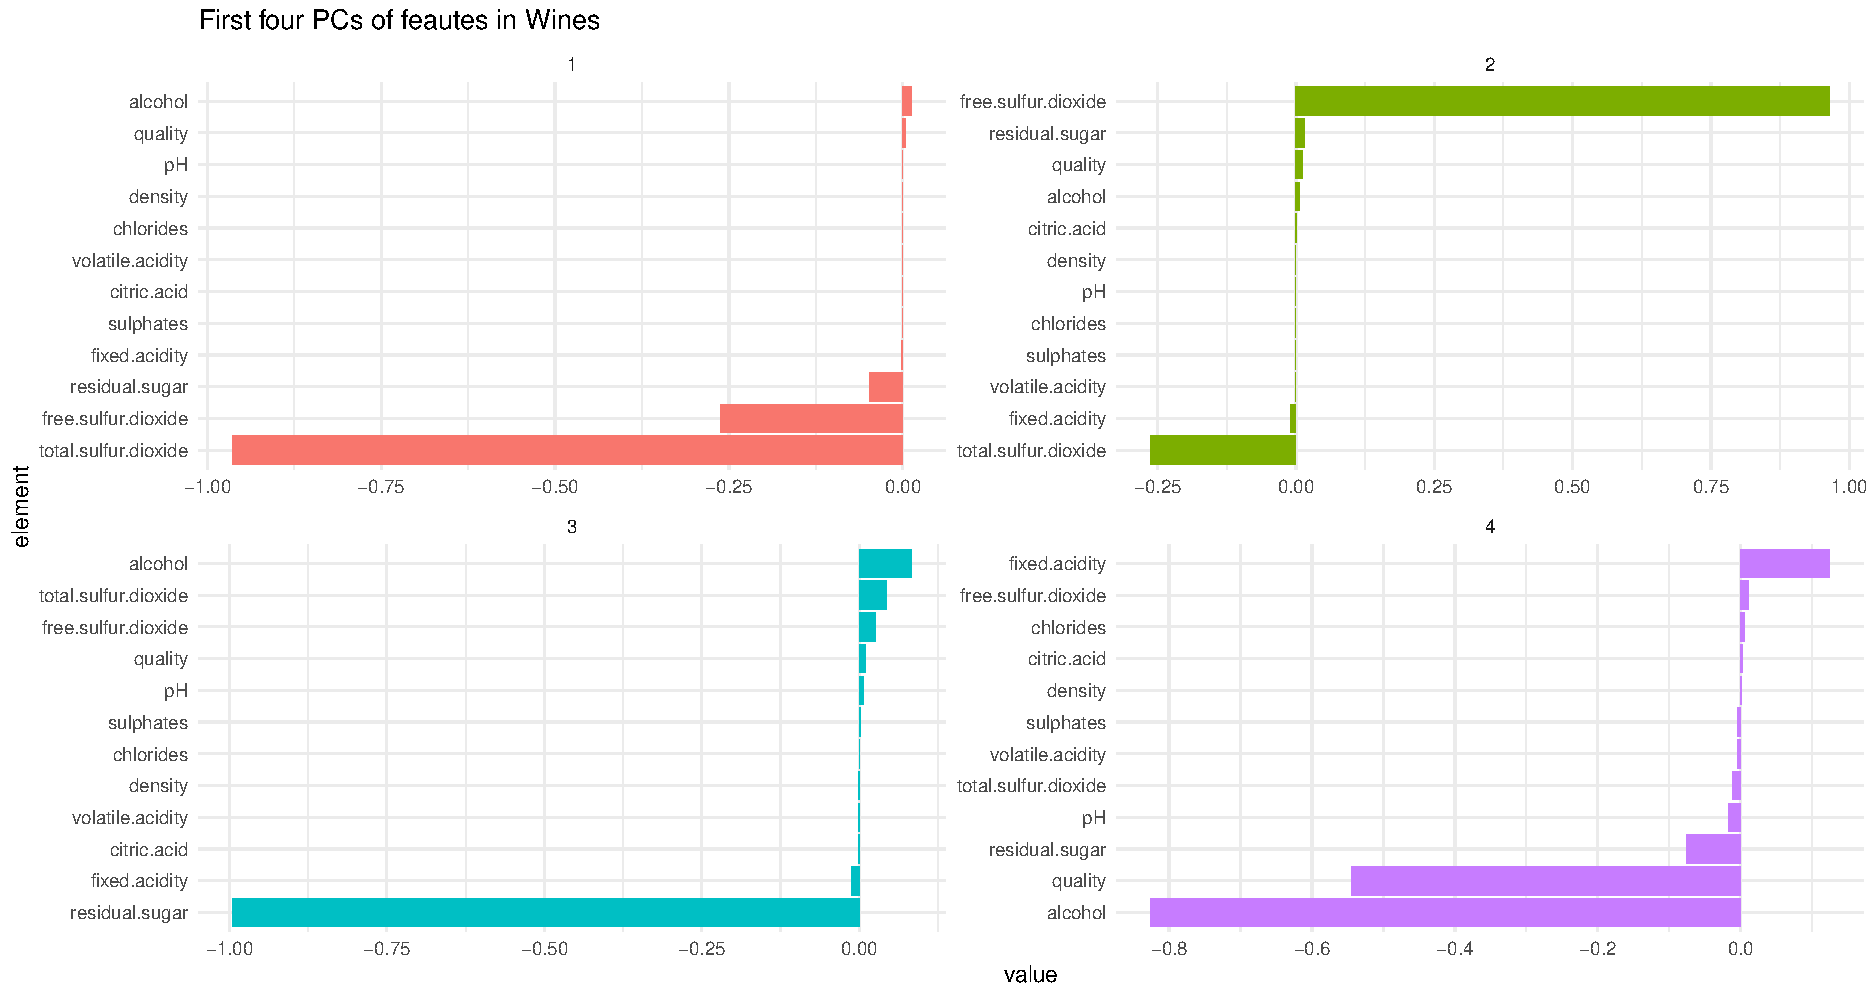
\includegraphics[width=\textwidth]{./output/1.b.pca-features.pdf}
\caption{centered image}
\end{figure}
\label{fig:pca_f}
\vspace{2em}
%----------

In \autoref{pca_f} the first four principal components are visualized along with the loadings of each columns. By on the two most extreme positive and negative values of the loadings, we can interpret the components into new kinds of variables. 

\begin{itemize}
\item PC1: Alcohol vs Sulfur Dioxide (free and total)
\item PC2: Free Sulfur Dioxide vs Total Sulfur Dioxide
\item PC3: Alcohol vs Sugar
\item PC4: Alcohol vs Acidity
\end{itemize}

It is clear that this dimensionality reduction technique produces results that reflect the real word. Sulfure Dioxide is a vital component in wine making as it regulates bacteria growth among other important tasks, yet, it also gives unpleasent oddors and tastes to the wine. PCA immidiately captures that reality by assigning the two biggest negative loadings on sulfure dioxide concentration (both free and total) to the first pricnipal component. In addition to that, the second most important component in order to classify the wines, is the origin of that Sulfure Dioxide. The total Sulfure Dioxide is the Free Sulfure Dioxide plus Sulfure Dioxide that is bound to other ingredients such as sugars etc. After investigating how much SO2 a wine has, as well as were it comes from (free vs total), the next most important factors have to do with the specific taste of the wine, mainly how sweet and how acidic the taste the wine has. 

We can now visualize the first two pricnipal components on a plot, while also coloring the datapoint according to their \textit{type}, the target variable. 
%----------
\vspace*{1em}
\begin{figure}[!h]
\centering
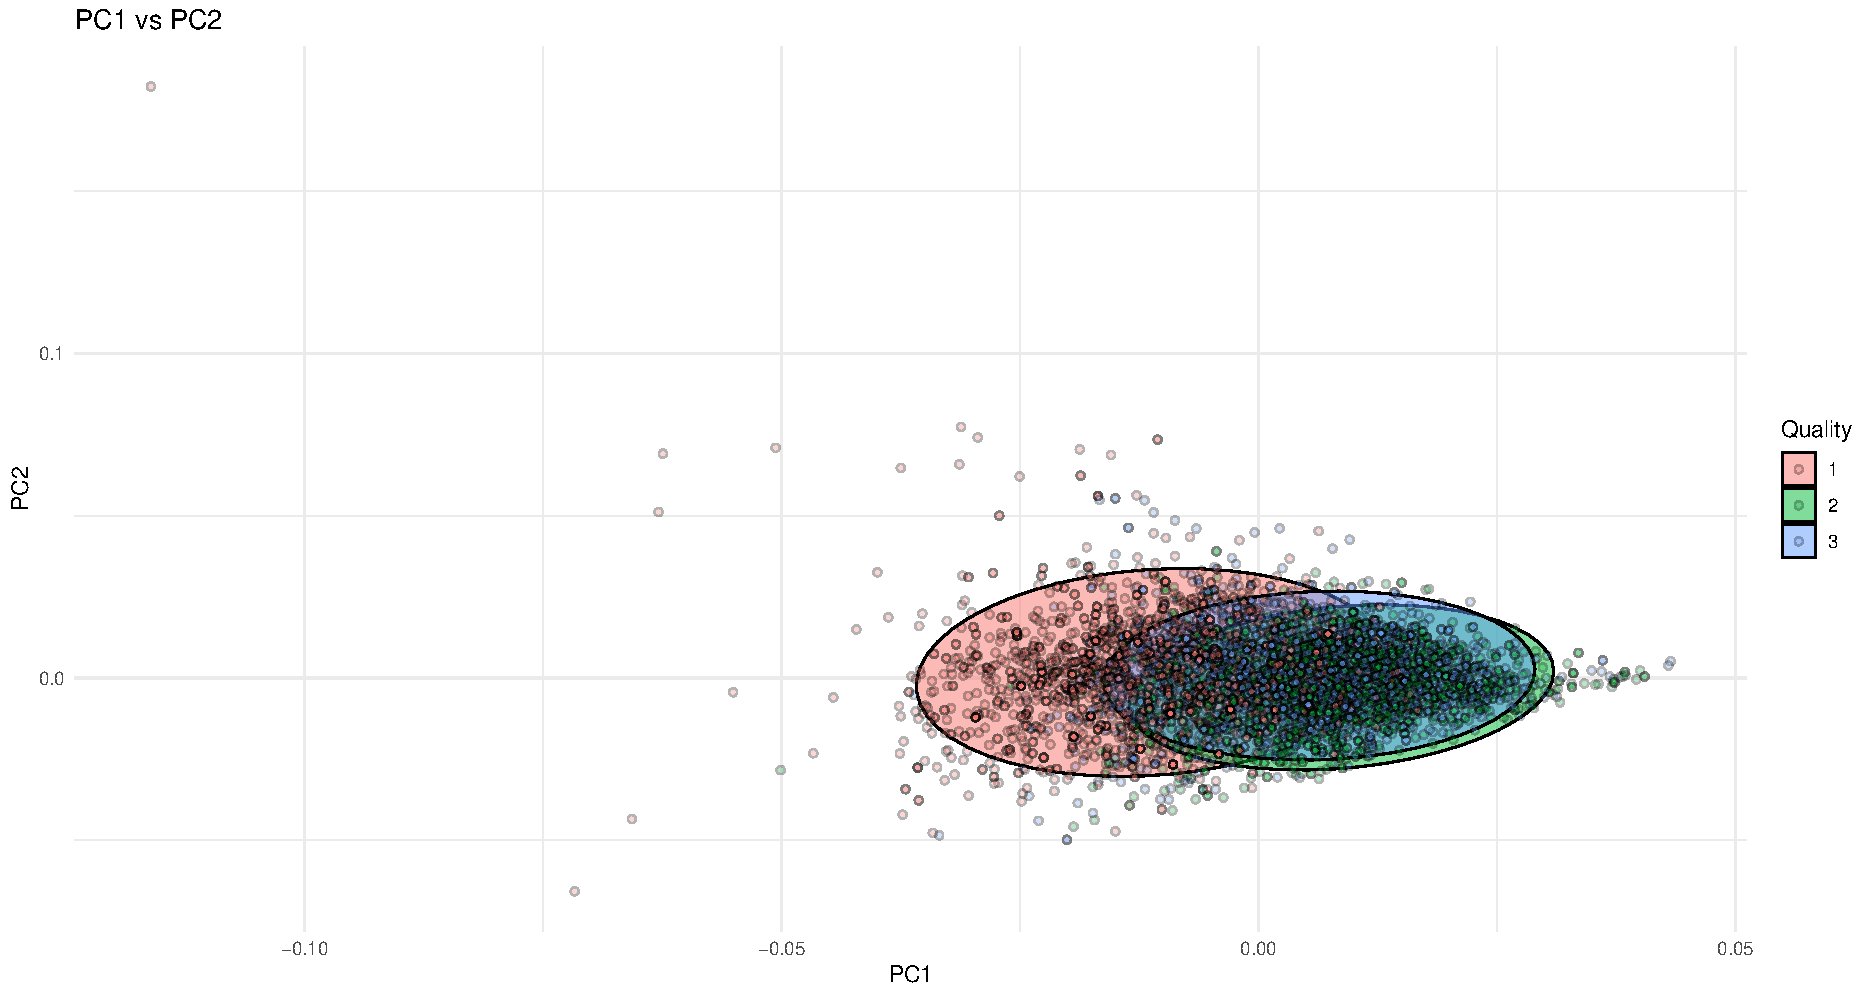
\includegraphics[width=\textwidth]{./output/1.c.pca-biplot.pdf}
\caption{centered image}
\label{fig:pca_biplot}
\end{figure}
\vspace{2em}
%----------
It is immidiately clear by \autoref{fig:pca_biplot} that \textit{type} classes two and three, have an extensive overlap in this graph. That is a useful information in the model evaluation, as we expect the model to "find it difficult" to distinguish a wine of type two from a wine of type three, while simultaneously having better accuracy in predicing class one. However, there a second major takeaway from \textit{Figure 3}, and that is the existance of potential anomalies. While the majority of the points are centered around $(0,0)$, some points are geometrically far away from the others of the same class. 

\subsubsection{t-SNE}
\label{sec:tsne}

Princiapal Component Analysis through singular value decomposition produced important findings and deepened our undestanding of the dataset. However, it was clear by \textit{Figure 3}, that it could not produce a clear enough separation between the classes. This could be because of the nature of the dataset, or it means that PCA is too simple to capture the complexity of the dataset, due to its linear nature. 

Therefore, a second, non-linear technique was tried in order to produce the corresponding figure as \textit{Figure 3}. This technique, is based on calculating the distances from each point to each neighbords and imposing a t-distribution on those values. It is an iterative algorithms that many times produces very good clustering.  However, in \autoref{fig:sne_biplot}, it is clear that \textit{type} classes two and three are still clustered together, while class one, is separated. 

The main takeaway from this analysis is that the dataset, although clean and simple in nature to understand, is mode complicated than it looks. This suggest that a simple model such as logistic regression might not be the model of choice. Neural Networks are a good candiate for such task due to their flexible nature. 

%----------
\vspace*{1em}
\begin{figure}[!h]
\centering
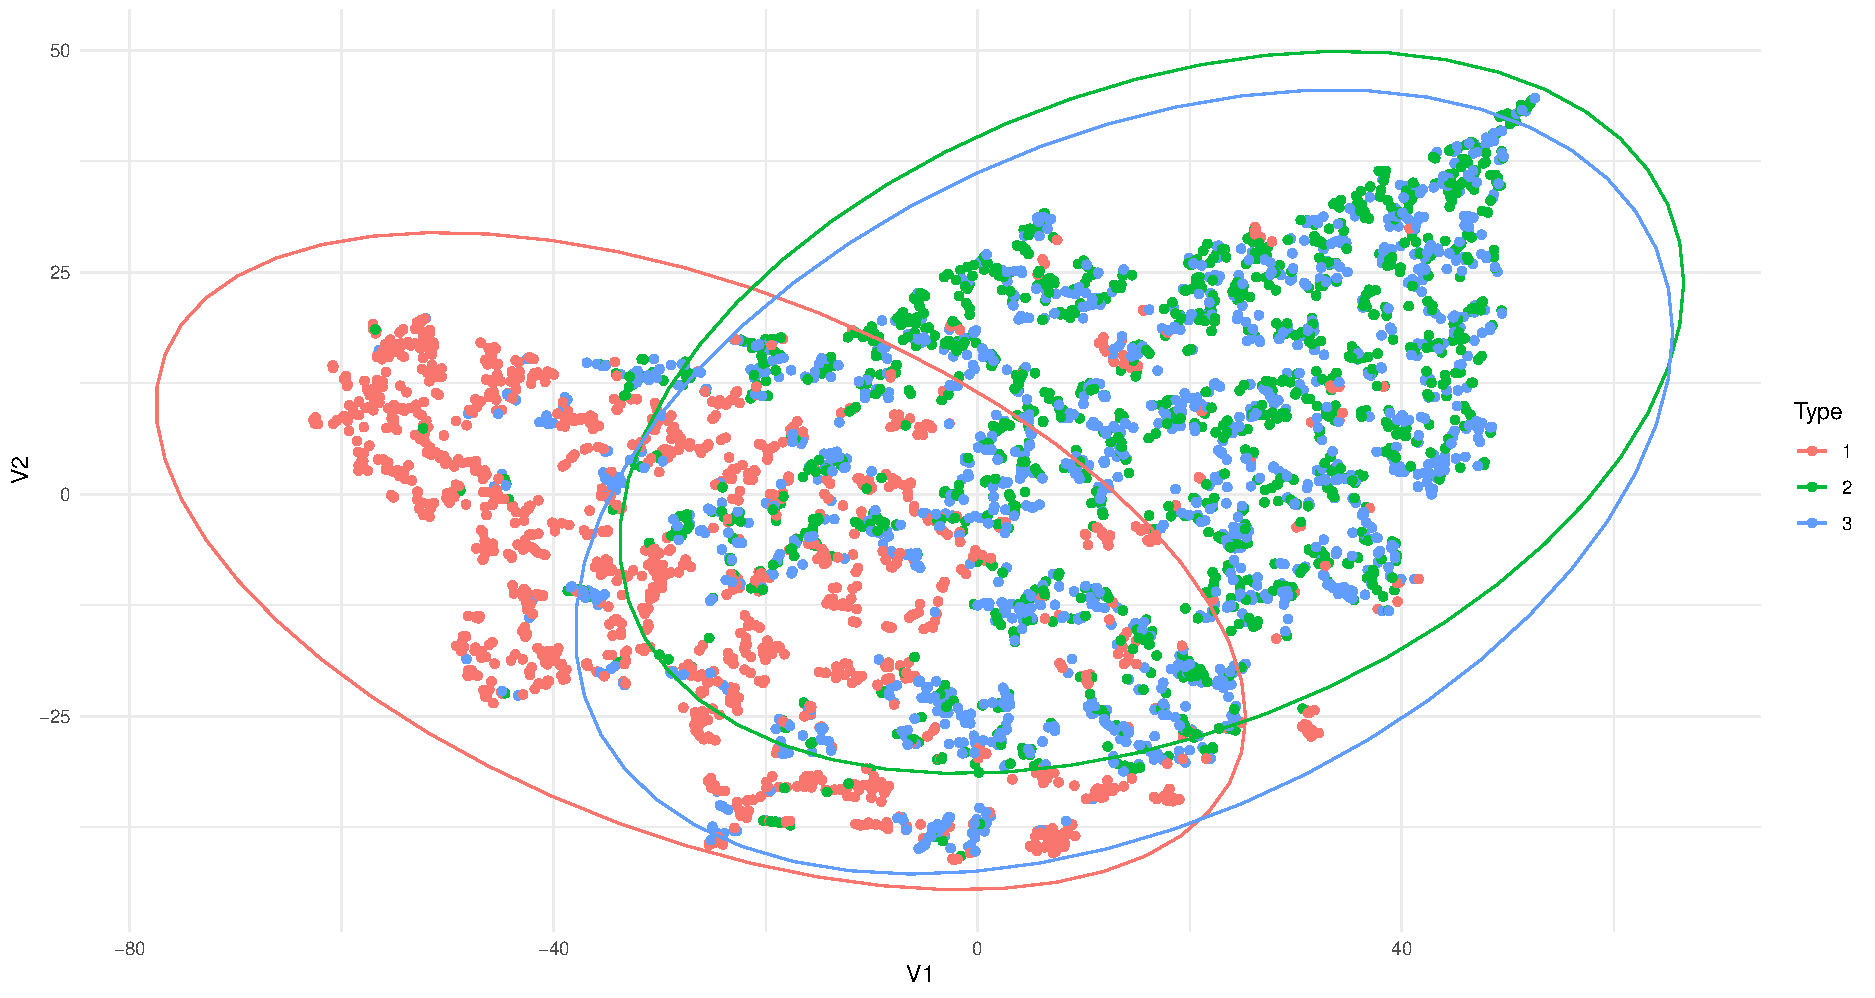
\includegraphics[width=\textwidth]{./output/1.d.t-sne.pdf}
\caption{centered image}
\label{fig:sne_biplot}
\end{figure}
\vspace{2em}
%----------


\subsection{Multivariate Analysis}
\label{sec:multivariate}

With the information revealed from PCA, we can now plot the highest and the lowest loadings of the four principal components, for each level of the target variable. The reason for plotting this graph is to investigate wheather some level of the \textit{type} variable, behaves different that the others when plotted on the same axis. 

%----------
\vspace*{1em}
\begin{figure}[!h]
\centering
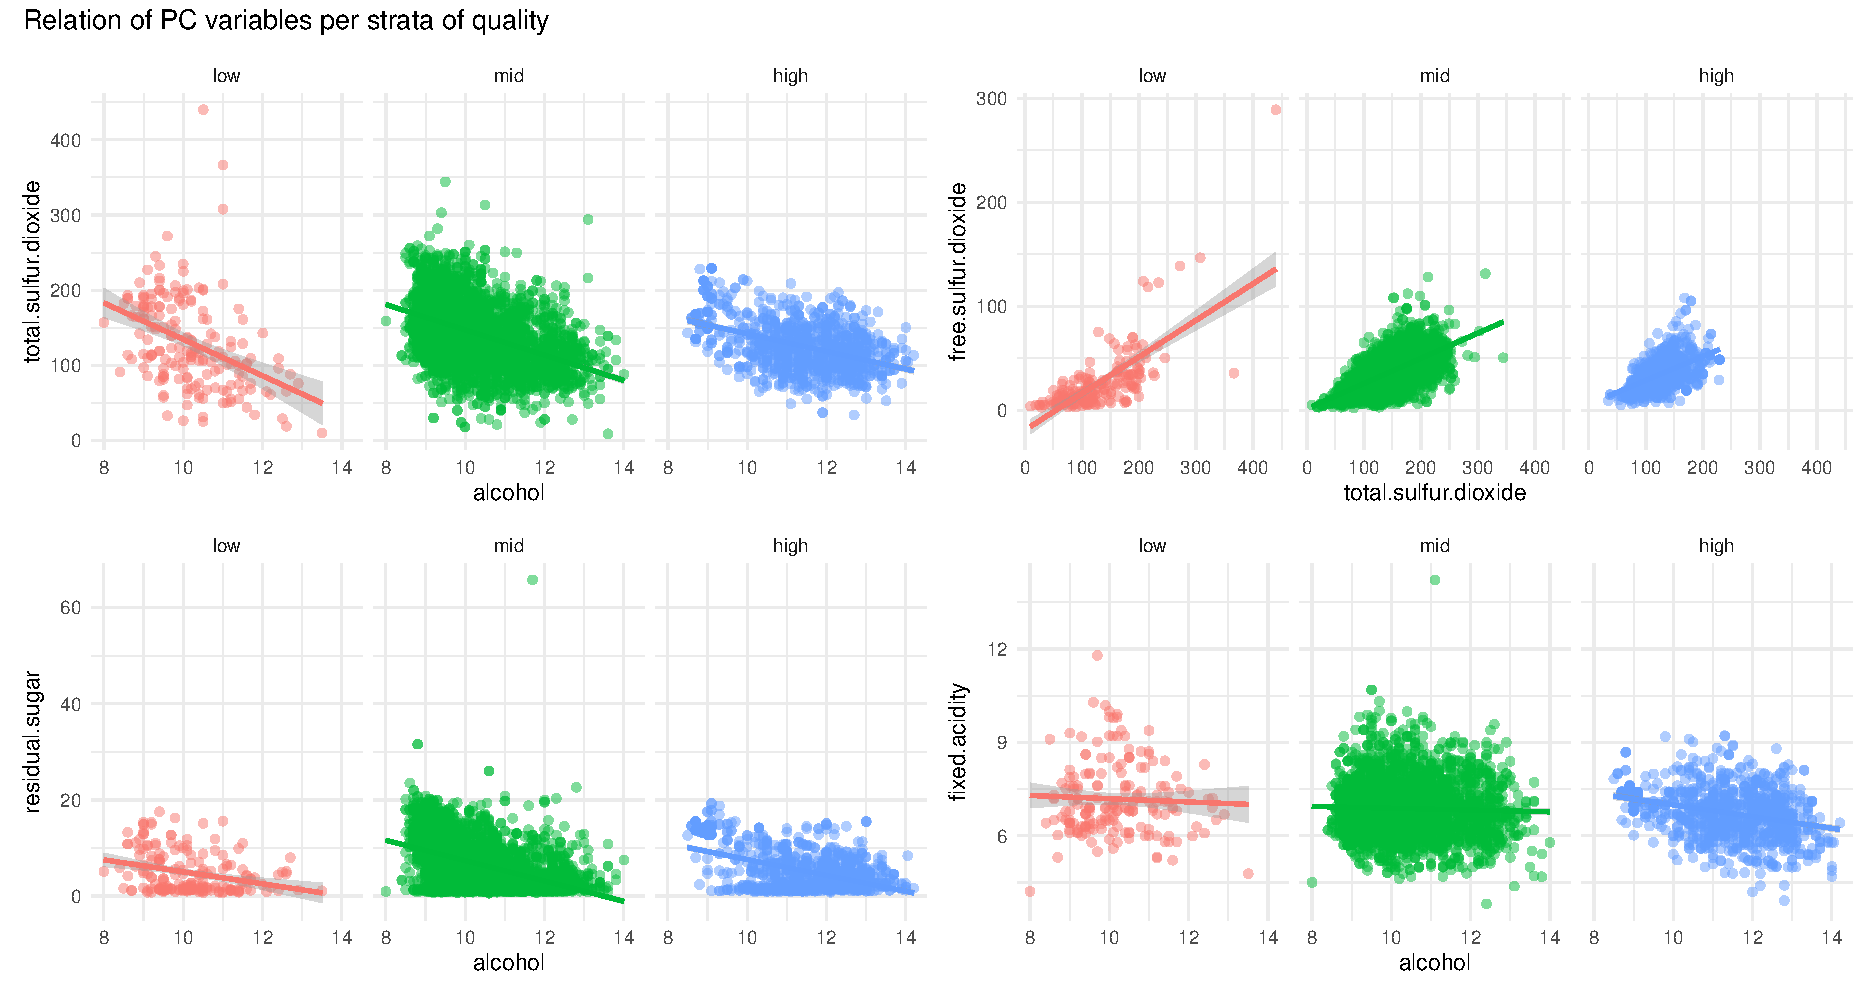
\includegraphics[width=\textwidth]{./output/1.g.multivariate-analysis.pdf}
\caption{}
\label{fig:multi}
\end{figure}
\vspace{2em}
%----------

In all four subplots of \autoref{fig:multi} we identify the same exact behaviour. The coefficient of the regression is negative on the \textit{total.sulfure.dioxide} against \textit{alcohol} axis for all levels, positive on the \textit{total.sulfure.dioxide} against \textit{free.sulfure.dioxide} axis, and close to zero for the other two PC scores. This finding, while not very exciting, is important, because it confirms once again that the relationship of our target variable \textit{type} and the features identified at the dimensionality reduction stage (\textit{total.sulfure.dioxide}, \textit{free.sulfure.dioxide}, \textit{alcohol}, \textit{residual.sugar}, and \textit{fixed.acidity}) are important for establishing a good model.

% ------------------------------------------------------------------------------------------------------
\section{Models}
\label{sec:methods}
In this section, the methods used to create the model will be discussed. This includes, the baseline model that is deterministic in nature, as well as the various Bayesian approaches. Firstly, the reason to choose neural networks as the model of choice, is due to the complexity of the research question, in combination with the complexity of the dataset as demostrated from the exploratory data analysis. Secondly, the Bayesian approach is important to make the neural network prediction \textit{stochastic}. 

In order to train the model and produce both high accuracy on the training and validation sets, as well as generalize well on the test set, a series of actions had to be taken. Firstly, a set of hyperparameters had been set for all models. Those hyperparameters are:

\begin{itemize}
\item The Learning Rate - ranging from $1e-1$ to $1e-8$ 
\item The number of layers between the Input and the Output - ranging from $2$ to $8$ 
\item The activation function of these layers - where the choices where:
\begin{itemize}
\item Rectified Linear Unit (reLU): $f(x) = \max(0,x)$
\item Exponential Linear Unit (ELU): $f(x) = \max(e^x-1,x)$
\item Sigmoid: $f(x)=\frac{1}{1+e^{-x}}$
\end{itemize}
\item The number of units in each function - rangin from $32$ to $512$, with a step of $128$
\end{itemize} 

The optimization process, was a \textsf{RandomSearch} algorithm, implemented with the \textsf{KerasTuner} package. This results in slightly different results in every run, however by switching to a \textsf{GridSearch} algorithm instead, the same outcome can be ensured each time. However, this process takes more time, since it is searching the whole hyperparameter space, while the \textsf{RandomSearch} takes less time to find the best model in each run. The metric used to judge which model is best was chosen to be \textit{accuracy}, due to its simplicity and suitability at the research problem. Lastly, the loss function that the models are minimizing in order to produce the best weights, was a custom made function that calculated the sum of the categorical crossentropy between the true and the predicted labels. The true labels have a known (for the traingin set) probability distribution (PMF), and the predicted labels, also have their own probability distribution (PMF). When the sum of the categorical crossentropies is minimum, it shows that the predicted PMF and the true PMF are as close as possible. Mathematically this is expresses as: 

\begin{equation}
\text{Loss} = \sum_{i=1}^{3} y_{true}^{(i)} \log{\frac{1}{y_{pred}^{(i)}}}  = -\sum_{i=1}^{3} y_{true}^{(i)} \log y_{pred}^{(i)} 
\end{equation}

Lastly, the models are trained for $2000$ training epochs. after a certain number of epochs, started to overfit. In order to avoid this pitfall, early stopping was implemented in the model with a patience of $200$ epochs. That means that if the validation accuracy, drops for $200$ epochs, the model assumes that it overfitted and stops trying to further minimize the loss function. This is why the x-axis varies in every Figure (\autoref{fig:base}, \autoref{fig:histories}, \autoref{fig:mcdrop}) where the history of accuracy per epoch is plotted. 

After the sucessful training of the base neural network, the predictions are deterministic. That means that each time a specific input is passed through the NN, the same output is produced. While this can be useful in certain applications, the goal of this project is to find a metric for the \textit{uncertainty} of the predictions. Thit is impossible to do with a deterministic process as samples cannot be drawn from  the posterior distribution to estimate it.  Therefore, after establishing a baseline, to prove that the problem can be solved with good enough accuracy, the network can become Bayesian by changing some of its layers to Bayesian layers. Afterwards, we can sample from the posterior distribution of the predictions, by predicting $n$ times the same input, in our case the test set. Then by storing each predicted probability (one for each class), in each draw ($1 \dots n$) we can compute average predictions, variances, confidence intervals, and more metrics discussed in \autoref{sec:results}. 

\subsection{Base Neural Network}
\label{sec:NN}

Before tackling the Bayesian Neural Network, a deterministic baseline should be first implemented. The model is built using the \textsf{keras} package for \textsf{Python}. The architecture the produced the best results is one with two hidden layers of $416$ and $160$ neurons respectively, densely connected to one another. This produces a total number of parameters to be estimated of $75,107$. The neural network is architecture depicted in \autoref{fig:base} (a).

\vspace*{1.5em}
\begin{figure}
\resizebox{.5\textwidth}{!}{%
\subfloat[Base Model Neural Network Architecture]
{\tikzset{every picture/.style={line width=0.75pt}} %set default line width to 0.75pt        
\begin{tikzpicture}[x=0.75pt,y=0.75pt,yscale=-1,xscale=1]
%uncomment if require: \path (0,329); %set diagram left start at 0, and has height of 329

%Shape: Rectangle [id:dp6981379495439248] 
\draw   (11,142.63) -- (50.93,142.63) -- (50.93,260.63) -- (11,260.63) -- cycle ;
%Shape: Rectangle [id:dp3116438864292579] 
\draw   (209,128.63) -- (248.93,128.63) -- (248.93,276.63) -- (209,276.63) -- cycle ;
%Shape: Rectangle [id:dp5504046010346768] 
\draw   (110,92.63) -- (149.93,92.63) -- (149.93,309.63) -- (110,309.63) -- cycle ;
%Straight Lines [id:da19613399481990768] 
\draw    (149.93,202.63) -- (205.93,202.63) ;
\draw [shift={(207.93,202.63)}, rotate = 180] [color={rgb, 255:red, 0; green, 0; blue, 0 }  ][line width=0.75]    (10.93,-3.29) .. controls (6.95,-1.4) and (3.31,-0.3) .. (0,0) .. controls (3.31,0.3) and (6.95,1.4) .. (10.93,3.29)   ;
%Straight Lines [id:da7665092917579182] 
\draw    (50.93,202.63) -- (106.93,202.63) ;
\draw [shift={(108.93,202.63)}, rotate = 180] [color={rgb, 255:red, 0; green, 0; blue, 0 }  ][line width=0.75]    (10.93,-3.29) .. controls (6.95,-1.4) and (3.31,-0.3) .. (0,0) .. controls (3.31,0.3) and (6.95,1.4) .. (10.93,3.29)   ;
%Straight Lines [id:da7866250847012999] 
\draw    (250.93,202.63) -- (306.93,202.63) ;
\draw [shift={(308.93,202.63)}, rotate = 180] [color={rgb, 255:red, 0; green, 0; blue, 0 }  ][line width=0.75]    (10.93,-3.29) .. controls (6.95,-1.4) and (3.31,-0.3) .. (0,0) .. controls (3.31,0.3) and (6.95,1.4) .. (10.93,3.29)   ;
%Shape: Rectangle [id:dp312756082115234] 
\draw   (308,156.12) -- (347.93,156.12) -- (347.93,250.12) -- (308,250.12) -- cycle ;

% Text Node
\draw (13,115) node [anchor=north west][inner sep=0.75pt]   [align=left] {Input};
% Text Node
\draw (206,103) node [anchor=north west][inner sep=0.75pt]   [align=left] {\begin{minipage}[lt]{32.19pt}\setlength\topsep{0pt}
\begin{center}
Dense
\end{center}

\end{minipage}};
% Text Node
\draw (106,65) node [anchor=north west][inner sep=0.75pt]   [align=left] {Dense};
% Text Node
\draw (21,237.4) node [anchor=north west][inner sep=0.75pt]    {$12$};
% Text Node
\draw (215,257.4) node [anchor=north west][inner sep=0.75pt]    {$160$};
% Text Node
\draw (115,288.4) node [anchor=north west][inner sep=0.75pt]    {$416$};
% Text Node
\draw (125,16) node [anchor=north west][inner sep=0.75pt]  [font=\large] [align=left] {\textbf{}};
% Text Node
\draw (304,133) node [anchor=north west][inner sep=0.75pt]   [align=left] {Output};
% Text Node
\draw (321,229.4) node [anchor=north west][inner sep=0.75pt]    {$3$};
\end{tikzpicture}}
}%
\subfloat[Base model History of epochs]
{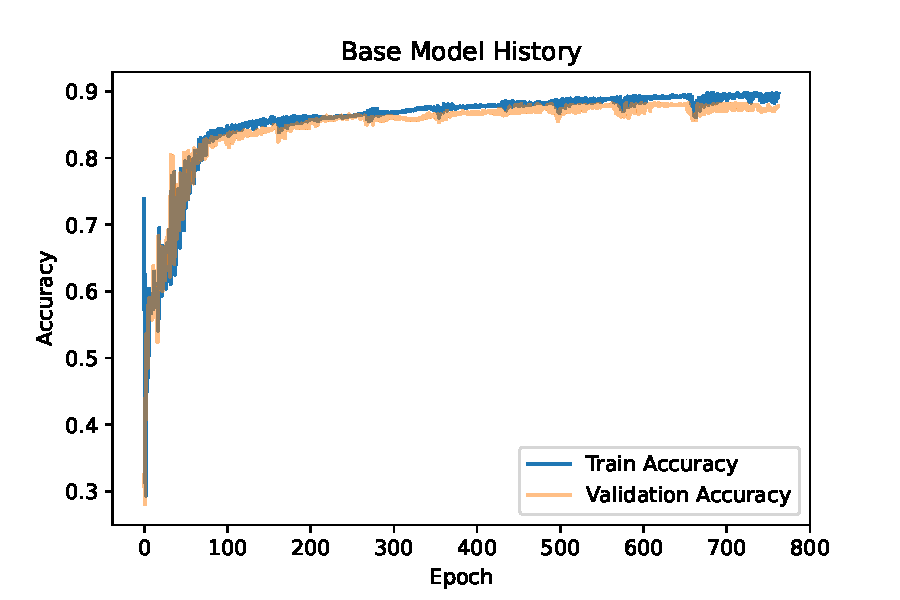
\includegraphics[width=.5\textwidth]{./output/2.a.history-base.pdf}}
\label{fig:base}
\caption{Baseline Architecture and Epoch History}
\end{figure}

\autoref{fig:base} (b) is a typical history of the training accuracy increasing over each epoch. Typicaly it stops before iteration $1000$ and the best accuracy of the model is close to $90\%$. This is a very good accuracy, since as we have seen at the exploratory data analysis, \textit{type 2} and \textit{type 3} are very difficult to distinguish. 

With the baseline model explained and trained, we gained an understanding at the extend to which the problem can be solved with neural networks. Arguably, an accuracy score of $90\%$ does not mean anything in a vaccum. $90\%$ accuracy in predictin a cetrain desease in a patient might be too low, while the same accuracy on an application less sensitive to important decision making might be exelent. However, in the specific task at question (classifying types of wines), this could be a good final score for the model. 

\subsection{Monte Carlo Dropout}
\label{sec:BNN}

Adding some Monte Carlo Dropout layers in the middle of each Dense layer, is the first approach in turning the base model into a Bayesian one. Simple dropout layers work during the training of the neural network, by randomly ignoring or "dropping out" a percentage of neurons along with the backward and forwand connections. This is being handled by random draws of a Bernoulli distribution with the "success" probability defined by the user. That process, still generates a \textit{deterministic} prediction, since at test time, which neurons are online is already decided. Monte Carlo dropout, is a wrapper of the simple dropout funciton that preserves the dropout at testing time. That way, the same prediction passed through the network twice, will produce different predictions according to which neurons and connections are online. Finally, these predictions are interpreted as random draws from the posterior distribution.

\vspace*{1.5em}
\begin{figure}
\resizebox{.5\textwidth}{!}{%
\subfloat[Monte Carlo Dropout NN Architecture]
{\tikzset{every picture/.style={line width=0.75pt}} %set default line width to 0.75pt        

\begin{tikzpicture}[x=0.75pt,y=0.75pt,yscale=-1,xscale=1]
%uncomment if require: \path (0,329); %set diagram left start at 0, and has height of 329

%Shape: Rectangle [id:dp6981379495439248] 
\draw   (11,142.63) -- (50.93,142.63) -- (50.93,260.63) -- (11,260.63) -- cycle ;
%Straight Lines [id:da21346322770194326] 
\draw    (50.93,201.63) -- (106.93,201.63) ;
\draw [shift={(108.93,201.63)}, rotate = 180] [color={rgb, 255:red, 0; green, 0; blue, 0 }  ][line width=0.75]    (10.93,-3.29) .. controls (6.95,-1.4) and (3.31,-0.3) .. (0,0) .. controls (3.31,0.3) and (6.95,1.4) .. (10.93,3.29)   ;
%Shape: Rectangle [id:dp29000115422593087] 
\draw   (108,125.63) -- (147.93,125.63) -- (147.93,276.63) -- (108,276.63) -- cycle ;
%Shape: Rectangle [id:dp3116438864292579] 
\draw   (209,128.63) -- (248.93,128.63) -- (248.93,276.63) -- (209,276.63) -- cycle ;
%Shape: Rectangle [id:dp5504046010346768] 
\draw   (308,92.63) -- (347.93,92.63) -- (347.93,309.63) -- (308,309.63) -- cycle ;
%Shape: Rectangle [id:dp2926920978374945] 
\draw   (412,95.63) -- (451.93,95.63) -- (451.93,309.63) -- (412,309.63) -- cycle ;
%Shape: Rectangle [id:dp43902801324987895] 
\draw   (512,156.63) -- (551.93,156.63) -- (551.93,248.63) -- (512,248.63) -- cycle ;
%Straight Lines [id:da19613399481990768] 
\draw    (149.93,202.63) -- (205.93,202.63) ;
\draw [shift={(207.93,202.63)}, rotate = 180] [color={rgb, 255:red, 0; green, 0; blue, 0 }  ][line width=0.75]    (10.93,-3.29) .. controls (6.95,-1.4) and (3.31,-0.3) .. (0,0) .. controls (3.31,0.3) and (6.95,1.4) .. (10.93,3.29)   ;
%Straight Lines [id:da7665092917579182] 
\draw    (248.93,202.63) -- (304.93,202.63) ;
\draw [shift={(306.93,202.63)}, rotate = 180] [color={rgb, 255:red, 0; green, 0; blue, 0 }  ][line width=0.75]    (10.93,-3.29) .. controls (6.95,-1.4) and (3.31,-0.3) .. (0,0) .. controls (3.31,0.3) and (6.95,1.4) .. (10.93,3.29)   ;
%Straight Lines [id:da00009484808513526843] 
\draw    (350.93,203.63) -- (406.93,203.63) ;
\draw [shift={(408.93,203.63)}, rotate = 180] [color={rgb, 255:red, 0; green, 0; blue, 0 }  ][line width=0.75]    (10.93,-3.29) .. controls (6.95,-1.4) and (3.31,-0.3) .. (0,0) .. controls (3.31,0.3) and (6.95,1.4) .. (10.93,3.29)   ;
%Straight Lines [id:da5648066531472558] 
\draw    (450.93,202.63) -- (506.93,202.63) ;
\draw [shift={(508.93,202.63)}, rotate = 180] [color={rgb, 255:red, 0; green, 0; blue, 0 }  ][line width=0.75]    (10.93,-3.29) .. controls (6.95,-1.4) and (3.31,-0.3) .. (0,0) .. controls (3.31,0.3) and (6.95,1.4) .. (10.93,3.29)   ;

% Text Node
\draw (7,104) node [anchor=north west][inner sep=0.75pt]   [align=left] {Dense};
% Text Node
\draw (104,91) node [anchor=north west][inner sep=0.75pt]   [align=left] {Dense};
% Text Node
\draw (211,84) node [anchor=north west][inner sep=0.75pt]   [align=left] {\begin{minipage}[lt]{24.81pt}\setlength\topsep{0pt}
\begin{center}
MC\\Drop
\end{center}

\end{minipage}};
% Text Node
\draw (414,49) node [anchor=north west][inner sep=0.75pt]   [align=left] {\begin{minipage}[lt]{24.81pt}\setlength\topsep{0pt}
\begin{center}
MC\\Drop
\end{center}

\end{minipage}};
% Text Node
\draw (304,65) node [anchor=north west][inner sep=0.75pt]   [align=left] {Dense};
% Text Node
\draw (510,134) node [anchor=north west][inner sep=0.75pt]   [align=left] {Dense};
% Text Node
\draw (21,237.4) node [anchor=north west][inner sep=0.75pt]    {$12$};
% Text Node
\draw (118,253.4) node [anchor=north west][inner sep=0.75pt]    {$32$};
% Text Node
\draw (219,254.4) node [anchor=north west][inner sep=0.75pt]    {$32$};
% Text Node
\draw (313,288.4) node [anchor=north west][inner sep=0.75pt]    {$160$};
% Text Node
\draw (417,289.4) node [anchor=north west][inner sep=0.75pt]    {$160$};
% Text Node
\draw (526,226.4) node [anchor=north west][inner sep=0.75pt]    {$3$};
% Text Node
\draw (161,10) node [anchor=north west][inner sep=0.75pt]  [font=\large] [align=left] {\textbf{Monte Carlo Dropout BNN}};
\end{tikzpicture}}
}%
\subfloat[Monte Carlo Dropout History of epochs]
{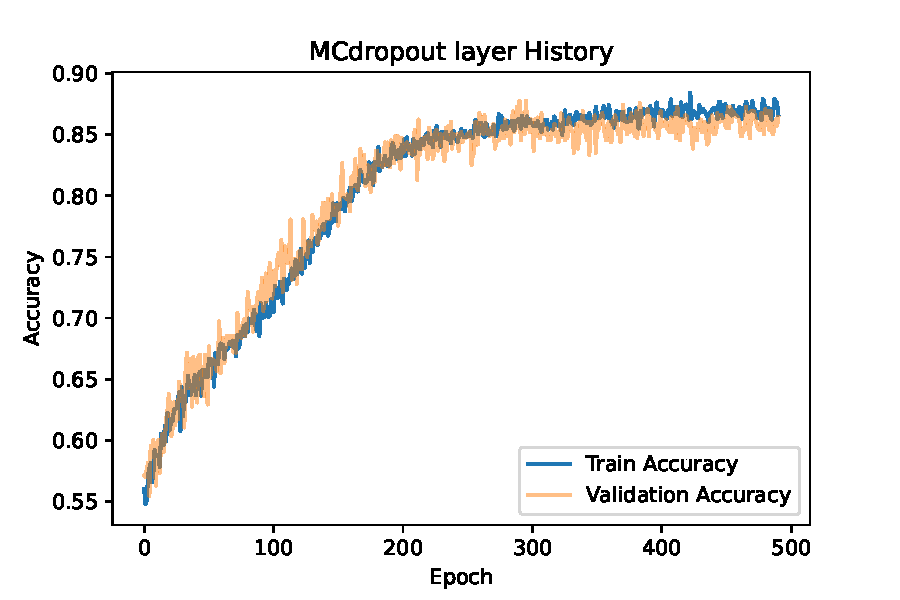
\includegraphics[width=.5\textwidth]{./output/2.d.history-mcdrop.pdf}}
\label{fig:mcdrop}
\caption{Monte Carlo Dropout Architecture and Epoch History}
\end{figure}

It is clear in \autoref{fig:mcdrop} (b) that there is a lot more variance in the prediction from epoch to epoch due to the random nature of the dropout layers. An important finding in this approach, is that the validation and the training accuracy are almost in all epochs at the same level. Contrary to the base model, where the validation accuracy increases with a slower rate than the training accuracy, this does not happen when the Monte Carlo Dropout layers are added to the model. It can even maintain for a short duration a higher validation accuracy than training accuracy, as seen from epochs $200$ to $400$ in \autoref{fig:mcdrop} (b) due to random chance.

\subsection{Other Bayesian Approaches}
\label{sec:other}
\blindtext

\tikzset{every picture/.style={line width=0.75pt}} %set default line width to 0.75pt        

\begin{tikzpicture}[x=0.75pt,y=0.75pt,yscale=-1,xscale=1]
%uncomment if require: \path (0,410); %set diagram left start at 0, and has height of 410

%Straight Lines [id:da7520912463319658] 
\draw    (210.86,-2.07) -- (208.93,407.35) ;
%Shape: Rectangle [id:dp6578673858538546] 
\draw   (282,67.5) -- (387.57,67.5) -- (387.57,101) -- (282,101) -- cycle ;
%Straight Lines [id:da17416205969228615] 
\draw    (333.57,100) -- (333.57,132.5) ;
\draw [shift={(333.57,134.5)}, rotate = 270] [color={rgb, 255:red, 0; green, 0; blue, 0 }  ][line width=0.75]    (10.93,-3.29) .. controls (6.95,-1.4) and (3.31,-0.3) .. (0,0) .. controls (3.31,0.3) and (6.95,1.4) .. (10.93,3.29)   ;
%Shape: Rectangle [id:dp9625306176469661] 
\draw   (271.57,133.5) -- (395.57,133.5) -- (395.57,167) -- (271.57,167) -- cycle ;
%Straight Lines [id:da12613771464913315] 
\draw    (334.57,167) -- (334.57,199.5) ;
\draw [shift={(334.57,201.5)}, rotate = 270] [color={rgb, 255:red, 0; green, 0; blue, 0 }  ][line width=0.75]    (10.93,-3.29) .. controls (6.95,-1.4) and (3.31,-0.3) .. (0,0) .. controls (3.31,0.3) and (6.95,1.4) .. (10.93,3.29)   ;
%Shape: Rectangle [id:dp8562897990585834] 
\draw   (263.57,200.5) -- (406.57,200.5) -- (406.57,234) -- (263.57,234) -- cycle ;
%Straight Lines [id:da4444814291856598] 
\draw    (334.57,233) -- (334.57,265.5) ;
\draw [shift={(334.57,267.5)}, rotate = 270] [color={rgb, 255:red, 0; green, 0; blue, 0 }  ][line width=0.75]    (10.93,-3.29) .. controls (6.95,-1.4) and (3.31,-0.3) .. (0,0) .. controls (3.31,0.3) and (6.95,1.4) .. (10.93,3.29)   ;
%Shape: Rectangle [id:dp48373983572684565] 
\draw   (263.57,266.5) -- (406.57,266.5) -- (406.57,300) -- (263.57,300) -- cycle ;
%Straight Lines [id:da014946150652792367] 
\draw    (334.57,299) -- (334.57,331.5) ;
\draw [shift={(334.57,333.5)}, rotate = 270] [color={rgb, 255:red, 0; green, 0; blue, 0 }  ][line width=0.75]    (10.93,-3.29) .. controls (6.95,-1.4) and (3.31,-0.3) .. (0,0) .. controls (3.31,0.3) and (6.95,1.4) .. (10.93,3.29)   ;
%Shape: Rectangle [id:dp37604395604633134] 
\draw   (267.57,332.5) -- (401.57,332.5) -- (401.57,366) -- (267.57,366) -- cycle ;
%Shape: Rectangle [id:dp3073637189530949] 
\draw   (498.57,69.5) -- (622.57,69.5) -- (622.57,103) -- (498.57,103) -- cycle ;
%Straight Lines [id:da8848887857143579] 
\draw    (561.57,102) -- (561.57,134.5) ;
\draw [shift={(561.57,136.5)}, rotate = 270] [color={rgb, 255:red, 0; green, 0; blue, 0 }  ][line width=0.75]    (10.93,-3.29) .. controls (6.95,-1.4) and (3.31,-0.3) .. (0,0) .. controls (3.31,0.3) and (6.95,1.4) .. (10.93,3.29)   ;
%Shape: Rectangle [id:dp4266654277213535] 
\draw   (508.57,135.5) -- (616.57,135.5) -- (616.57,169) -- (508.57,169) -- cycle ;
%Straight Lines [id:da06249075020880501] 
\draw    (563.57,304) -- (563.57,336.5) ;
\draw [shift={(563.57,338.5)}, rotate = 270] [color={rgb, 255:red, 0; green, 0; blue, 0 }  ][line width=0.75]    (10.93,-3.29) .. controls (6.95,-1.4) and (3.31,-0.3) .. (0,0) .. controls (3.31,0.3) and (6.95,1.4) .. (10.93,3.29)   ;
%Shape: Rectangle [id:dp7312721900848995] 
\draw   (513.57,337.5) -- (612.57,337.5) -- (612.57,371) -- (513.57,371) -- cycle ;
%Straight Lines [id:da5460497639581126] 
\draw    (561.57,169) -- (561.57,201.5) ;
\draw [shift={(561.57,203.5)}, rotate = 270] [color={rgb, 255:red, 0; green, 0; blue, 0 }  ][line width=0.75]    (10.93,-3.29) .. controls (6.95,-1.4) and (3.31,-0.3) .. (0,0) .. controls (3.31,0.3) and (6.95,1.4) .. (10.93,3.29)   ;
%Shape: Rectangle [id:dp26552065436119876] 
\draw   (494.57,202.5) -- (628.57,202.5) -- (628.57,236) -- (494.57,236) -- cycle ;
%Straight Lines [id:da7458999475229033] 
\draw    (561.57,237) -- (561.57,269.5) ;
\draw [shift={(561.57,271.5)}, rotate = 270] [color={rgb, 255:red, 0; green, 0; blue, 0 }  ][line width=0.75]    (10.93,-3.29) .. controls (6.95,-1.4) and (3.31,-0.3) .. (0,0) .. controls (3.31,0.3) and (6.95,1.4) .. (10.93,3.29)   ;
%Shape: Rectangle [id:dp5970670487921053] 
\draw   (508.57,270.5) -- (616.57,270.5) -- (616.57,304) -- (508.57,304) -- cycle ;
%Shape: Rectangle [id:dp010365484916174061] 
\draw   (37,67.93) -- (142.57,67.93) -- (142.57,101.43) -- (37,101.43) -- cycle ;
%Straight Lines [id:da435445969504787] 
\draw    (88.57,100.43) -- (88.57,132.93) ;
\draw [shift={(88.57,134.93)}, rotate = 270] [color={rgb, 255:red, 0; green, 0; blue, 0 }  ][line width=0.75]    (10.93,-3.29) .. controls (6.95,-1.4) and (3.31,-0.3) .. (0,0) .. controls (3.31,0.3) and (6.95,1.4) .. (10.93,3.29)   ;
%Shape: Rectangle [id:dp8334163094493718] 
\draw   (17.57,133.93) -- (161.57,133.93) -- (161.57,167.43) -- (17.57,167.43) -- cycle ;
%Straight Lines [id:da7154001058216675] 
\draw    (89.57,167.43) -- (89.57,199.93) ;
\draw [shift={(89.57,201.93)}, rotate = 270] [color={rgb, 255:red, 0; green, 0; blue, 0 }  ][line width=0.75]    (10.93,-3.29) .. controls (6.95,-1.4) and (3.31,-0.3) .. (0,0) .. controls (3.31,0.3) and (6.95,1.4) .. (10.93,3.29)   ;
%Shape: Rectangle [id:dp0885963983905822] 
\draw   (18.57,200.93) -- (161.57,200.93) -- (161.57,234.43) -- (18.57,234.43) -- cycle ;
%Straight Lines [id:da20534784584705146] 
\draw    (89.57,233.43) -- (89.57,265.93) ;
\draw [shift={(89.57,267.93)}, rotate = 270] [color={rgb, 255:red, 0; green, 0; blue, 0 }  ][line width=0.75]    (10.93,-3.29) .. controls (6.95,-1.4) and (3.31,-0.3) .. (0,0) .. controls (3.31,0.3) and (6.95,1.4) .. (10.93,3.29)   ;
%Shape: Rectangle [id:dp4577629971609587] 
\draw   (1.57,266.93) -- (177.57,266.93) -- (177.57,300.43) -- (1.57,300.43) -- cycle ;
%Straight Lines [id:da8408482777880153] 
\draw    (89.57,299.43) -- (89.57,331.93) ;
\draw [shift={(89.57,333.93)}, rotate = 270] [color={rgb, 255:red, 0; green, 0; blue, 0 }  ][line width=0.75]    (10.93,-3.29) .. controls (6.95,-1.4) and (3.31,-0.3) .. (0,0) .. controls (3.31,0.3) and (6.95,1.4) .. (10.93,3.29)   ;
%Shape: Rectangle [id:dp6122483307594775] 
\draw   (47.57,332.93) -- (131.57,332.93) -- (131.57,366.43) -- (47.57,366.43) -- cycle ;
%Curve Lines [id:da019301893461343367] 
\draw    (337,366) .. controls (490.93,516.62) and (456.93,-175.65) .. (559.93,72.53) ;
\draw [shift={(559.93,72.53)}, rotate = 247.45999999999998] [color={rgb, 255:red, 0; green, 0; blue, 0 }  ][line width=0.75]    (10.93,-3.29) .. controls (6.95,-1.4) and (3.31,-0.3) .. (0,0) .. controls (3.31,0.3) and (6.95,1.4) .. (10.93,3.29)   ;

% Text Node
\draw (293.57,76) node [anchor=north west][inner sep=0.75pt]   [align=left] {\textbf{Input}};
% Text Node
\draw (519.57,345.86) node [anchor=north west][inner sep=0.75pt]   [align=left] {\textbf{Flipout}};
% Text Node
\draw (593.57,345.26) node [anchor=north west][inner sep=0.75pt]    {$3$};
% Text Node
\draw (363.57,75.4) node [anchor=north west][inner sep=0.75pt]    {$12$};
% Text Node
\draw (273.57,143) node [anchor=north west][inner sep=0.75pt]   [align=left] {Flipout};
% Text Node
\draw (267.57,210) node [anchor=north west][inner sep=0.75pt]   [align=left] {Dense};
% Text Node
\draw (267.57,276) node [anchor=north west][inner sep=0.75pt]   [align=left] {Dense};
% Text Node
\draw (271.57,341) node [anchor=north west][inner sep=0.75pt]   [align=left] {Dense};
% Text Node
\draw (501.57,78) node [anchor=north west][inner sep=0.75pt]   [align=left] {Dense};
% Text Node
\draw (507.57,143) node [anchor=north west][inner sep=0.75pt]   [align=left] {Dense};
% Text Node
\draw (364.57,143.4) node [anchor=north west][inner sep=0.75pt]    {$416$};
% Text Node
\draw (375.57,210.4) node [anchor=north west][inner sep=0.75pt]    {$160$};
% Text Node
\draw (371.57,276.4) node [anchor=north west][inner sep=0.75pt]    {$416$};
% Text Node
\draw (368.57,341.4) node [anchor=north west][inner sep=0.75pt]    {$416$};
% Text Node
\draw (591.57,78.4) node [anchor=north west][inner sep=0.75pt]    {$288$};
% Text Node
\draw (587.57,144.4) node [anchor=north west][inner sep=0.75pt]    {$160$};
% Text Node
\draw (498.57,211) node [anchor=north west][inner sep=0.75pt]   [align=left] {Dense};
% Text Node
\draw (595.57,211.4) node [anchor=north west][inner sep=0.75pt]    {$416$};
% Text Node
\draw (507.57,278) node [anchor=north west][inner sep=0.75pt]   [align=left] {Dense};
% Text Node
\draw (587.57,279.4) node [anchor=north west][inner sep=0.75pt]    {$160$};
% Text Node
\draw (286.57,9) node [anchor=north west][inner sep=0.75pt]  [font=\small] [align=left] {\begin{minipage}[lt]{65.92pt}\setlength\topsep{0pt}
\begin{center}
\textbf{Dense Flipout }\\\textbf{BNN}
\end{center}

\end{minipage}};
% Text Node
\draw (30,9.71) node [anchor=north west][inner sep=0.75pt]  [font=\small] [align=left] {\begin{minipage}[lt]{78.7pt}\setlength\topsep{0pt}
\begin{center}
\textbf{Variational Layer }\\\textbf{BNN}
\end{center}

\end{minipage}};
% Text Node
\draw (48.57,76.43) node [anchor=north west][inner sep=0.75pt]   [align=left] {\textbf{Input}};
% Text Node
\draw (118.57,75.83) node [anchor=north west][inner sep=0.75pt]    {$12$};
% Text Node
\draw (20.57,144.43) node [anchor=north west][inner sep=0.75pt]   [align=left] {Variational};
% Text Node
\draw (22.57,210.43) node [anchor=north west][inner sep=0.75pt]   [align=left] {Dense};
% Text Node
\draw (6.57,275.43) node [anchor=north west][inner sep=0.75pt]   [align=left] {Dense};
% Text Node
\draw (51.57,342.43) node [anchor=north west][inner sep=0.75pt]   [align=left] {\textbf{Output}};
% Text Node
\draw (128.57,143.83) node [anchor=north west][inner sep=0.75pt]    {$288$};
% Text Node
\draw (130.57,210.83) node [anchor=north west][inner sep=0.75pt]    {$288$};
% Text Node
\draw (146.57,276.83) node [anchor=north west][inner sep=0.75pt]    {$416$};
% Text Node
\draw (119.57,341.83) node [anchor=north west][inner sep=0.75pt]    {$3$};


\end{tikzpicture}



\begin{figure}[]
    \centering
    \subfloat[Variational layers History of epochs]
    {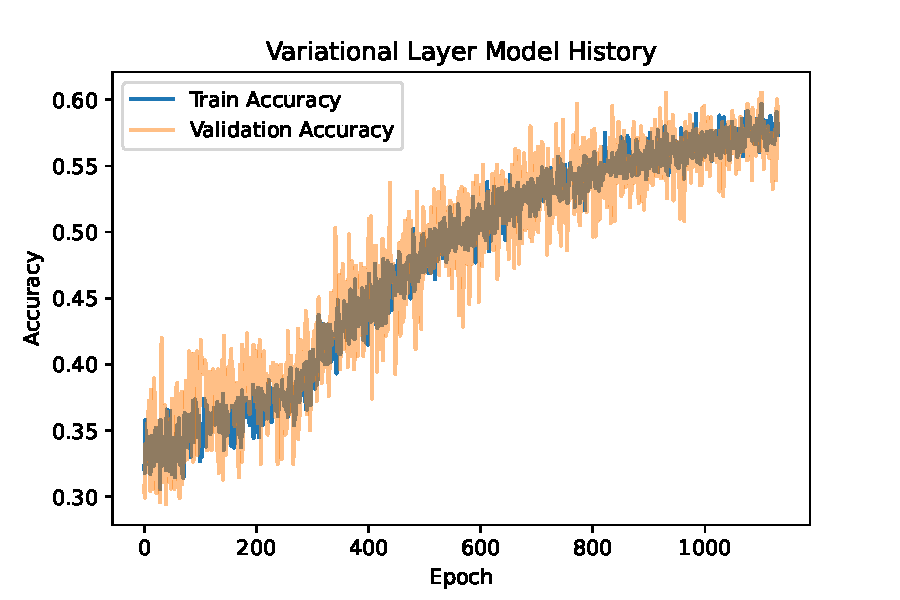
\includegraphics[width=.5\textwidth]{./output/2.b.history-var.pdf}}
    \subfloat[Flipout layers History of epochs]
    {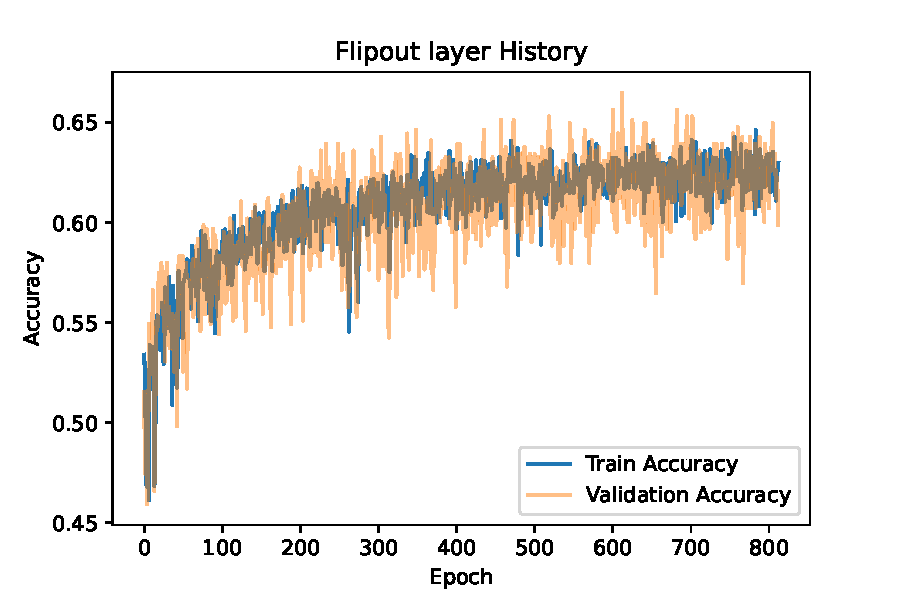
\includegraphics[width=.5\textwidth]{./output/2.c.history-flip.pdf}}
    \caption{History of other Bayesian Models (Flipout and Dense Variational)}
    \label{fig:histories}
\end{figure}

\subsection{Model Validation}
\label{sec:validation}
\blindtext

%----------
\vspace*{1em}
\begin{figure}[!h]
\centering
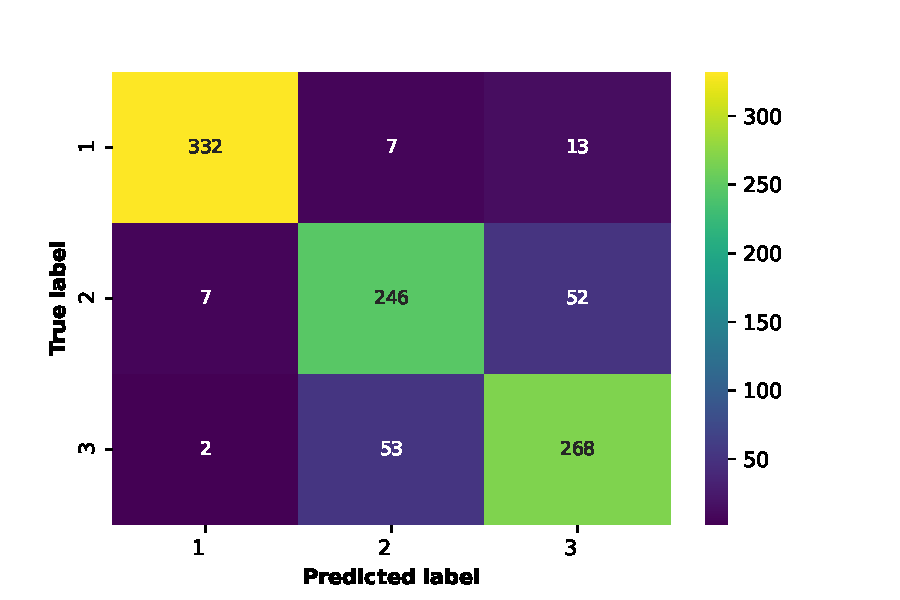
\includegraphics[width=\textwidth]{./output/2.e.confmat-base.pdf}
\caption{}
\label{fig:mcdrop}
\end{figure}
\vspace{2em}
%----------

\begin{figure}[!h]
    \centering
    \subfloat[Class 1 Explanation]
    {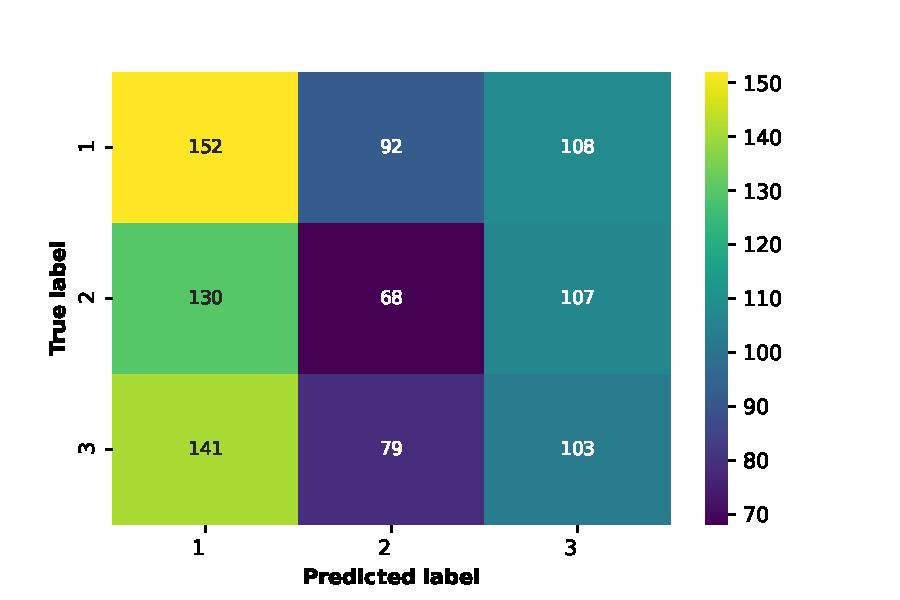
\includegraphics[width=.33\textwidth]{./output/2.f.confmat-var.pdf}}
    \subfloat[Class 2 Explanation]
    {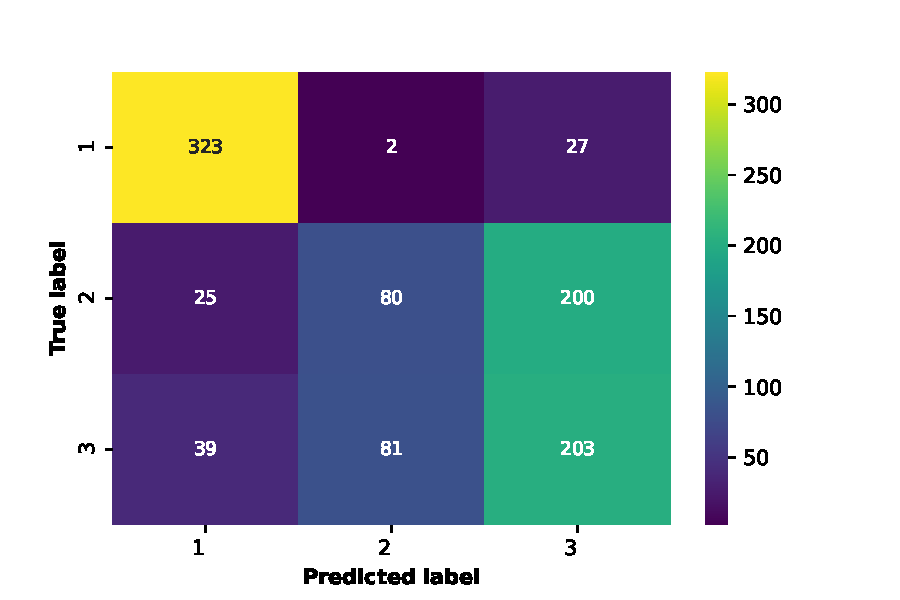
\includegraphics[width=.33\textwidth]{./output/2.g.confmat-flip.pdf}}
    \subfloat[Class 3 Explanation]
    {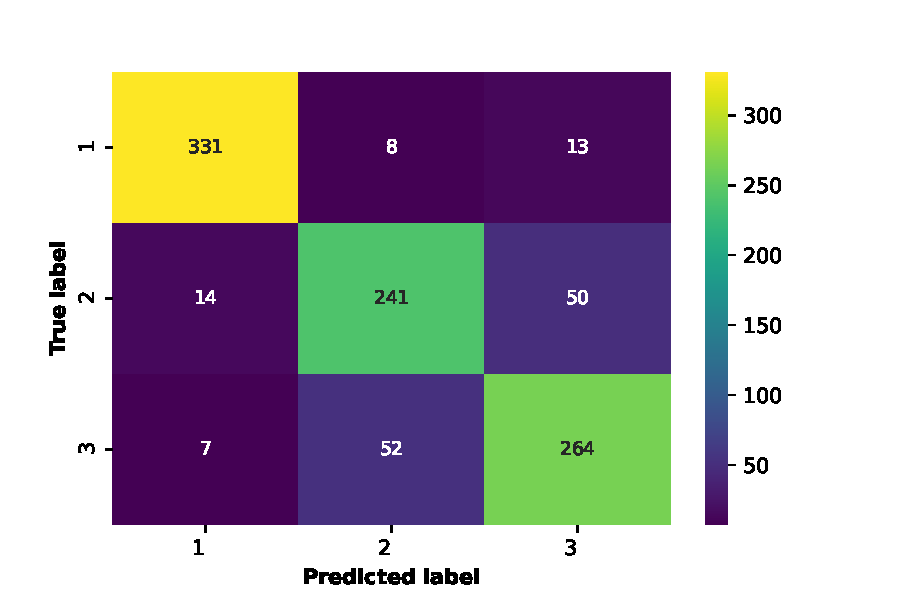
\includegraphics[width=.33\textwidth]{./output/2.h.confmat-mcdrop.pdf}}
    \caption{}
    \label{fig:shap_exp}
\end{figure}

\subsection{Model Explanation}
\label{sec:explanation}
\blindtext

%----------
\vspace*{1em}
\begin{figure}[!h]
\centering
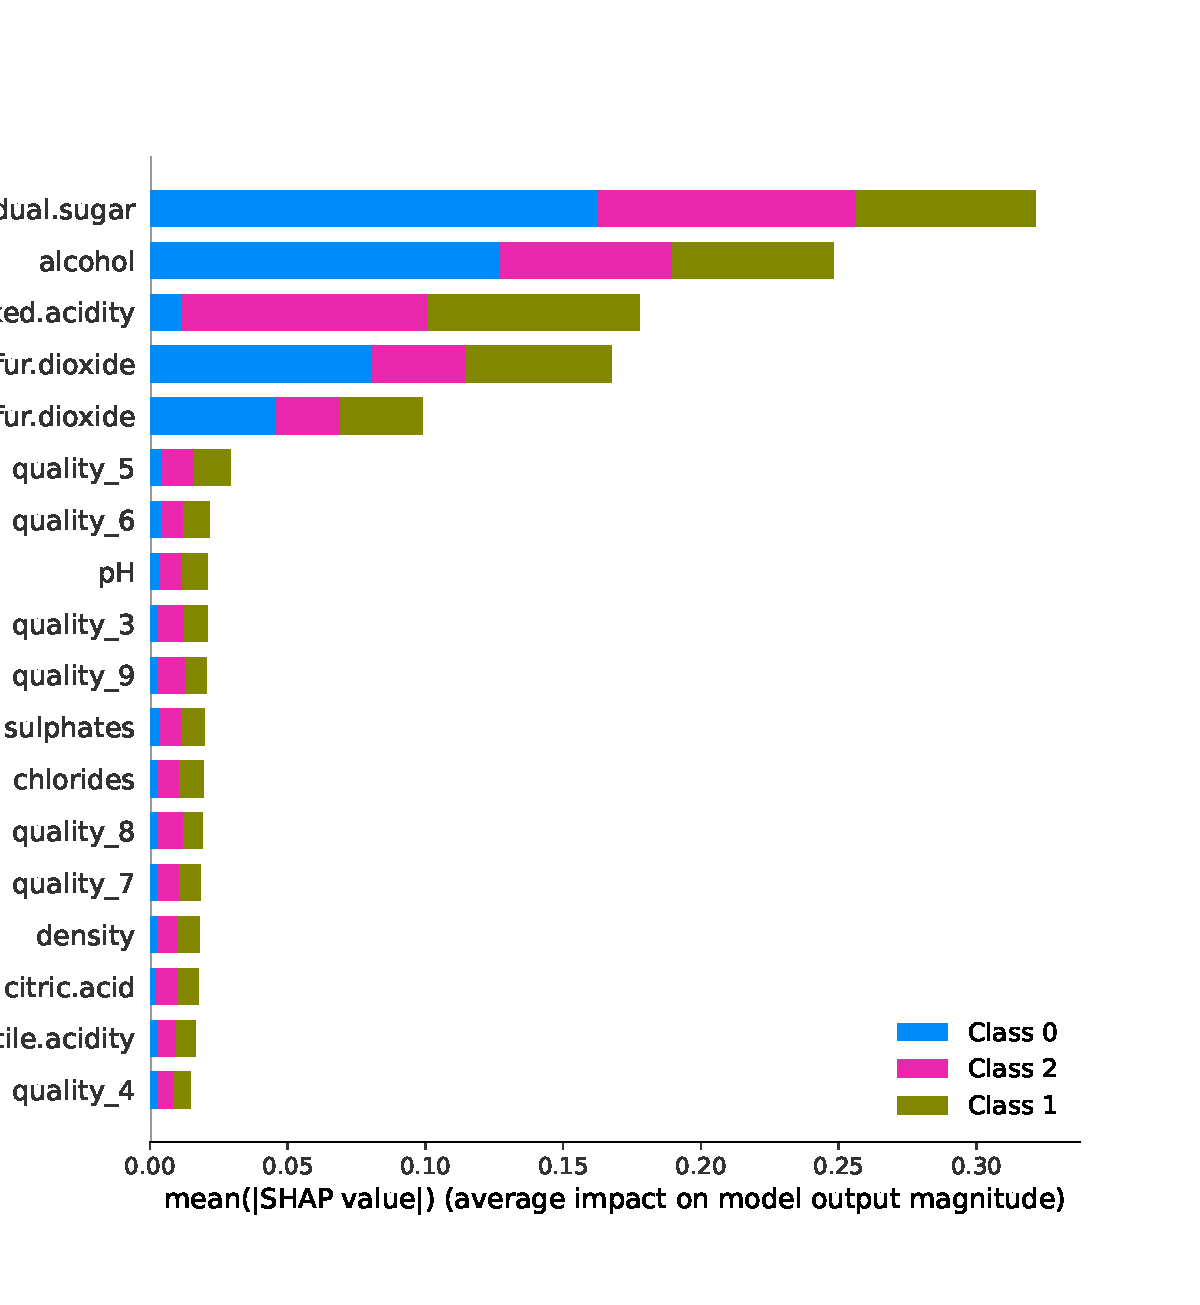
\includegraphics[width=\textwidth]{./output/2.i.shap-summary.pdf}
\caption{}
\label{fig:shap_sum}
\end{figure}
\vspace{2em}
%----------

\begin{figure}[!h]
    \centering
    \subfloat[Class 1 Explanation]
    {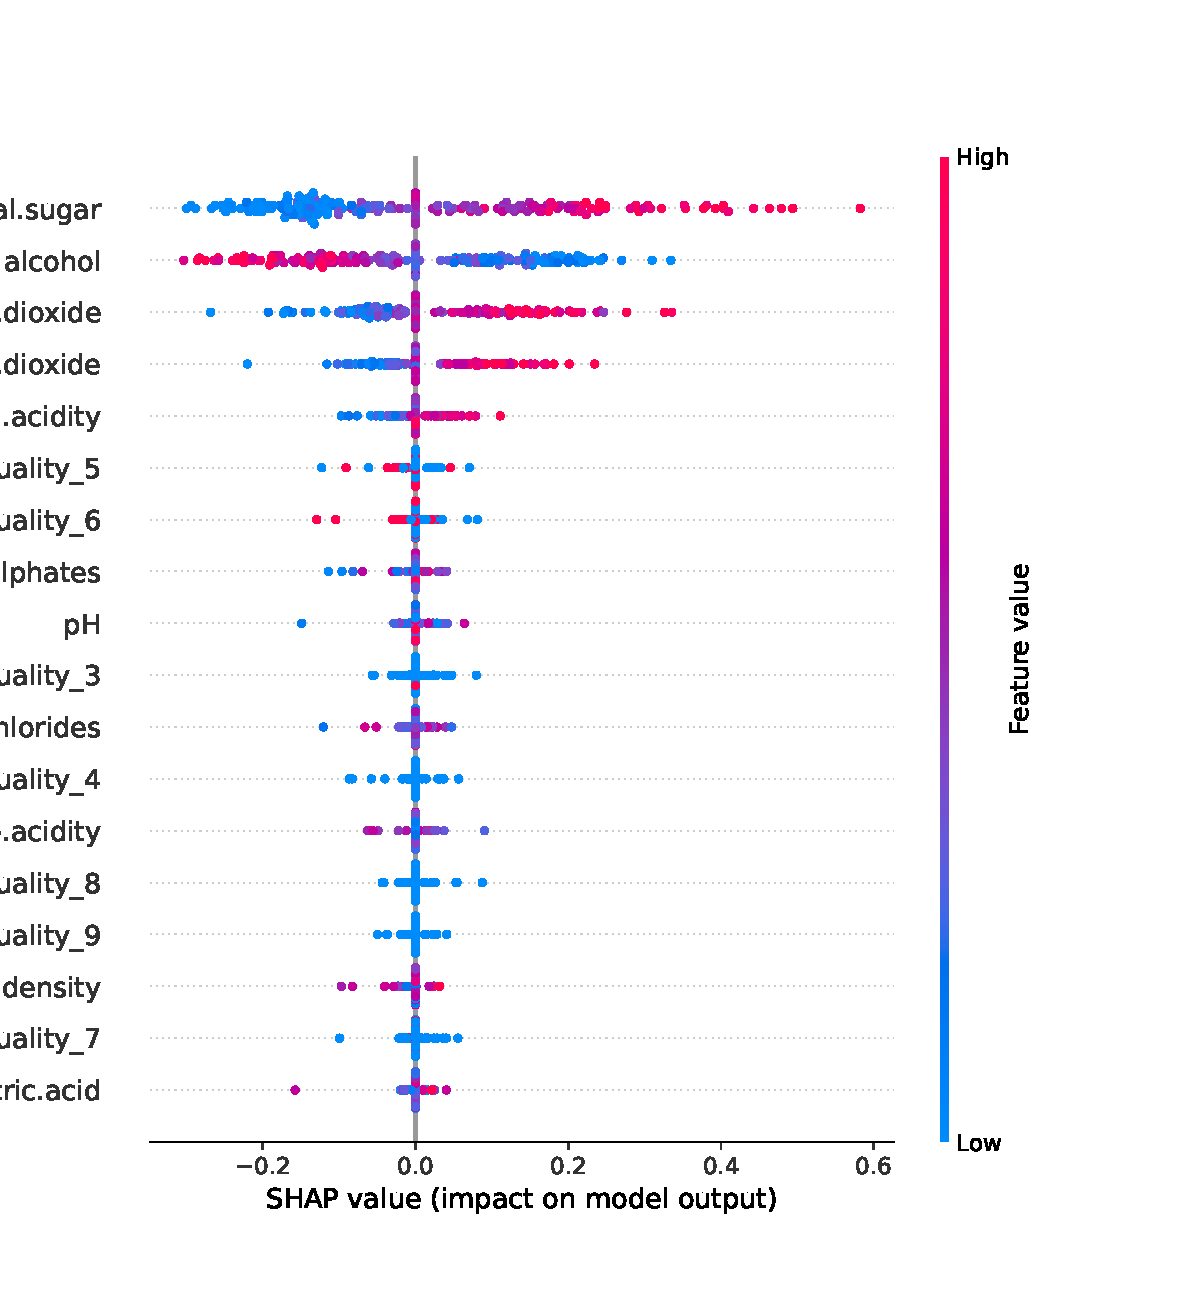
\includegraphics[width=.33\textwidth]{./output/2.j.shap-class0.pdf}}
    \subfloat[Class 2 Explanation]
    {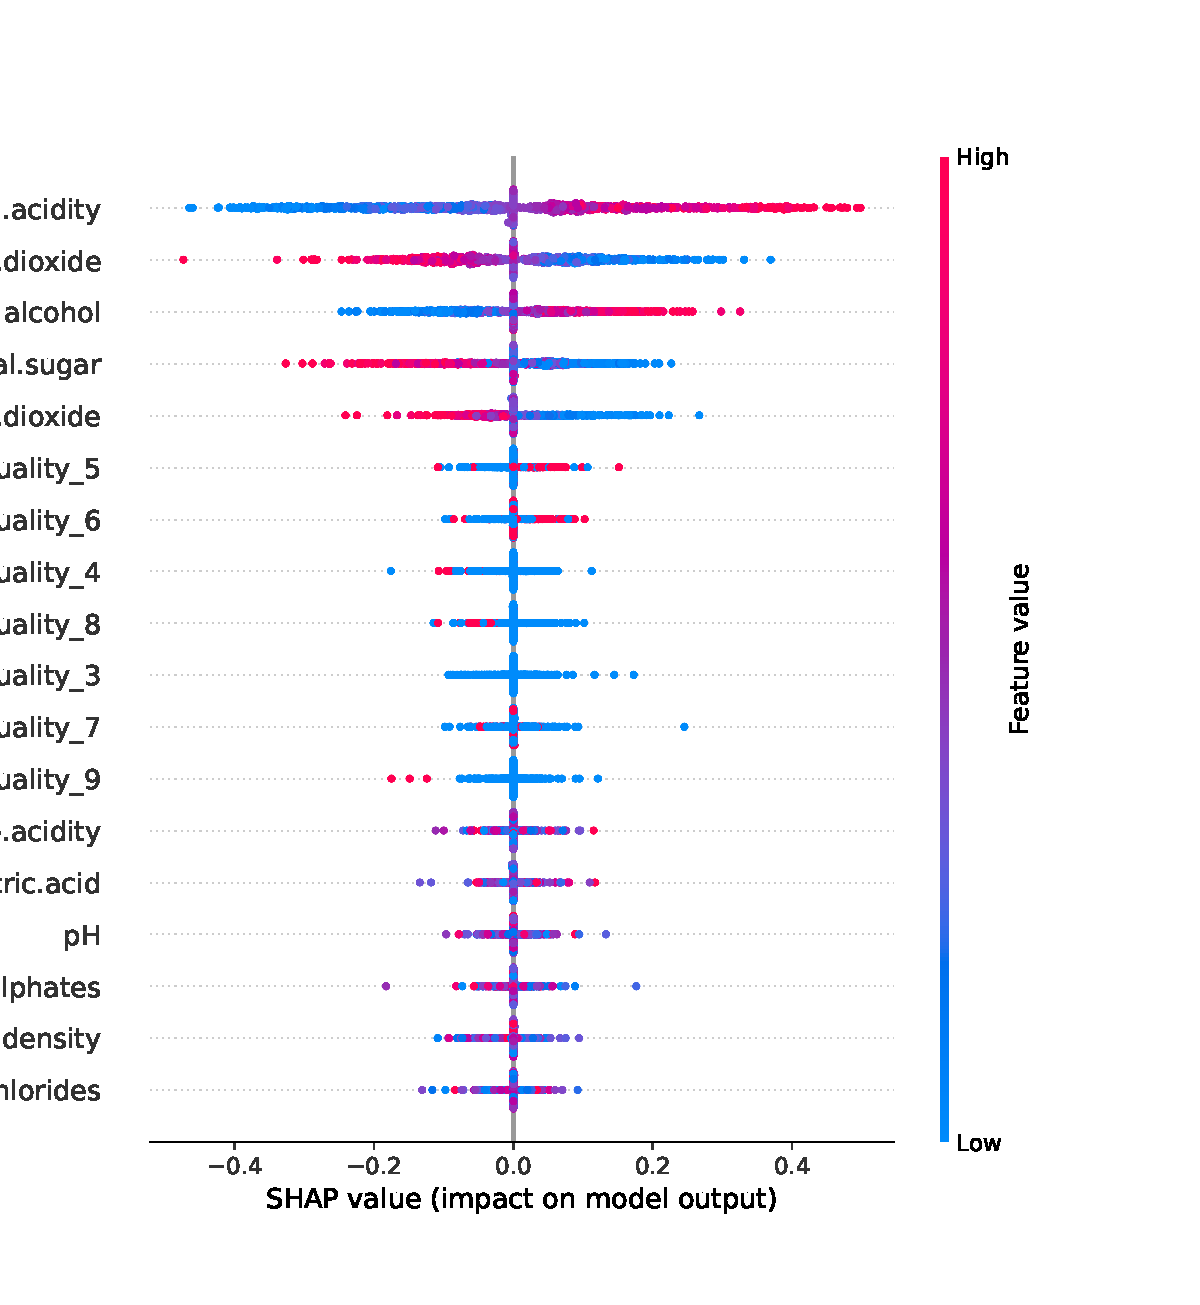
\includegraphics[width=.33\textwidth]{./output/2.k.shap-class1.pdf}}
    \subfloat[Class 3 Explanation]
    {
\includegraphics[width=.33\textwidth]{./output/2.l.shap-class2.pdf}}
    \caption{}
    \label{fig:shap_exp}
\end{figure}

% ------------------------------------------------------------------------------------------------------
\section{Results}
\label{sec:results}
\blindtext

\subsection{Standard Deviation}
\blindtext

\subsection{Confidence Intervals}
\blindtext

\subsection{Entropy}
\begin{figure}[!ht]
\centering
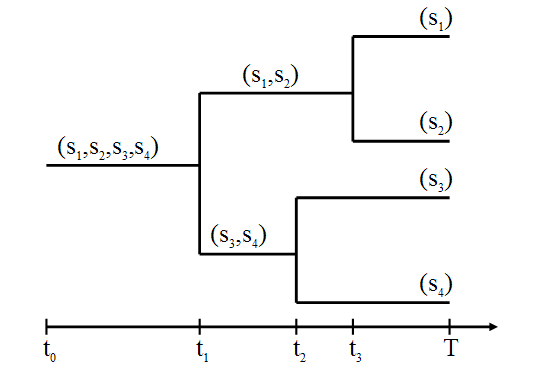
\includegraphics[width=8cm]{scenTree.png}
\caption{Look at this scenario tree with funny times $t_{1}$ and scenarios $s_{1}$ etc.}
\label{fig:scenarioTree}
\end{figure}

\cleardoublepage

% ------------------------------------------------------------------------------------------------------
\section{Discussion}
\blindtext
\clearpage

% ------------------------------------------------------------------------------------------------------
%tliterature.bib
\bibliography{literature}
\clearpage

% ------------------------------------------------------------------------------------------------------
\appendix
\section*{Appendices}
\addcontentsline{toc}{section}{Appendices}
\blindtext

\section{Appendix first topic}
\label{app:one}
\blindtext

\section{Appendix second topic}
\label{app:one}
\blindtext
\clearpage

\end{document}
